\chapter{Chemical Reaction Equilibrium}\label{Chapter:ChemicalReactions}

   \begin{LearningObjectivesBlock}{Learning Objectives}
      Upon completion of this chapter, you will be able to
        \begin{enumerate}
           \item 
        \end{enumerate}
\medskip
     Recommended reading: Chapters 13 of \citet{SmithVanNess_Book}, 8 of \cite{Sandler_Book}, 12 of \citet{Lue_Book}, 14 of \citet{Moran_Book}, 11 of \citet{Devoe_Book} or 7 of \citet{Atkins_Book}.
   \end{LearningObjectivesBlock}


%%%%%%%%%%%%%%%%%%%%%%%%%%%%%%%%%%%%%%%%%%%%%%%%%%%%%%%%%%%%%%%%%
\begin{comment}
   \begin{LearningObjectivesBlock}{Learning Objectives}
      Upon completion of this chapter, you will be able to
        \begin{enumerate}
           \item {\bf Knowledge:} Define, Name, Select, State 
           \item {\bf Comprehension:} Describe, Identify, Discuss
           \item {\bf Application:} Apply, Demonstrate, Employ, Sketch
           \item {\bf Analysis:} Analyse, Compare, Calculate, Solve
           \item {\bf Synthesis:} Determine, Formulate
           \item {\bf Evaluation:} Assess, Check, Estimate, Compare, Measure, Monitor
        \end{enumerate}
\end{comment}
%%%%%%%%%%%%%%%%%%%%%%%%%%%%%%%%%%%%%%%%%%%%%%%%%%%%%%%%%%%%%%%%%

%%%% ETOC
\localtableofcontents
   
%%% SECTION
\section{Introduction}\label{Chapter:ChemicalReactions:Section:Introduction}
In previous Chapters, we studied the thermodynamic behaviour of gases and liquids at equilibrium conditions assuming that species do not react. However, in many industrial, environmental and bio-medical applications, chemical reactions are the driving force behind important processes.
      \begin{wrapfigure}{r}{0.5\textwidth}%{figure}[hpt]
         \begin{center}
           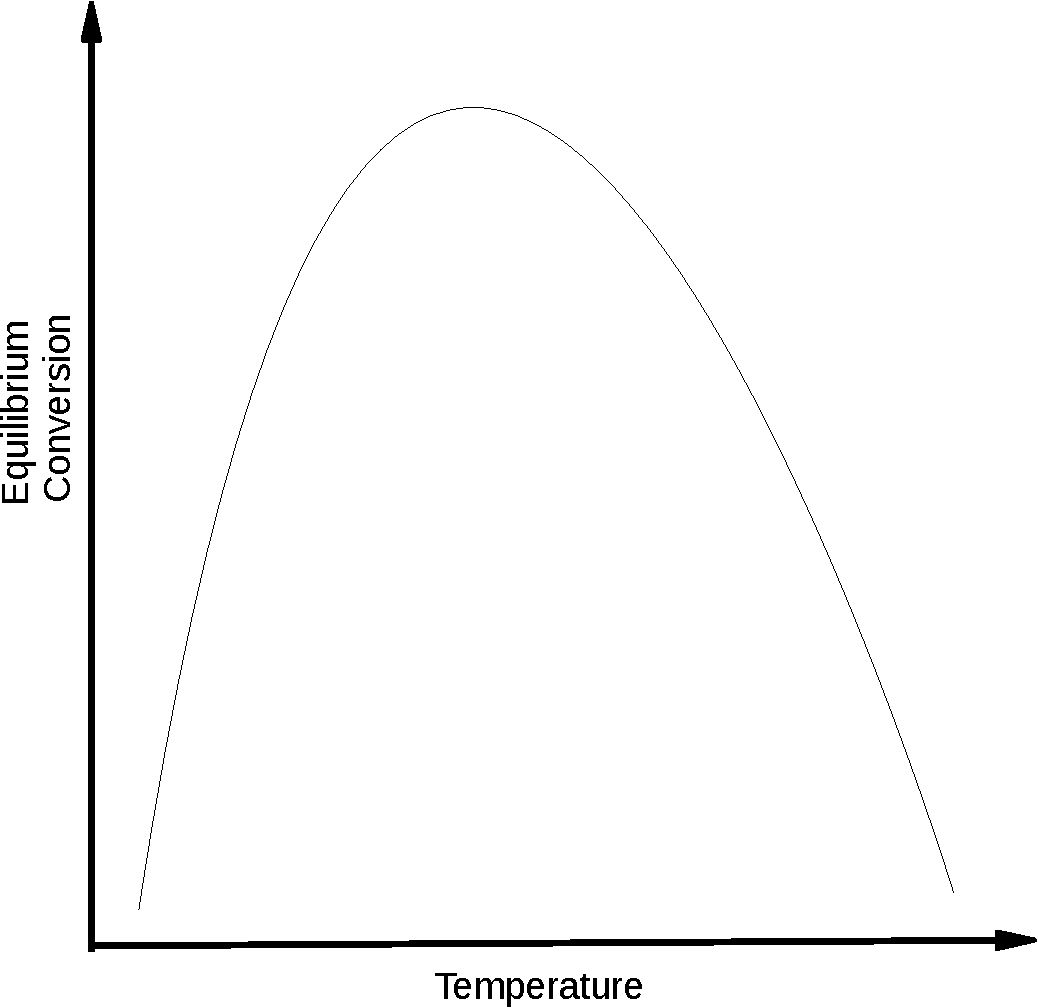
\includegraphics[width=0.5\columnwidth,clip]{./Figs/Mod06_SchematicEqReaction_Temp_b}
           \caption{Sketch of equilibrium reaction and temperature.}\label{Mod06Fig01}
         \end{center}
       \end{wrapfigure}%{figure}
      Reactive systems are often characterised in terms of the maximum possible yield of the target product(s) at prescribed conditions, starting from the reactants (\ie raw materials). From {\it chemical kinetics} theory, rates of reaction and the reaction mechanisms\footnote{Here, it is important to define two terms commonly used in chemical kinetics theory:
        \begin{enumerate}[a)]
           \item {\it rate of reaction}: changes in the reactants concentrations with time, $\mfr[C]{}{\text{react}}=\mfr[C]{}{\text{react}}(t)$ (\ie `speed' of the reaction) and,
           \item {\it mechanisms of reactions}: stages of the reaction (in molecular level) that leads to the consumption of reactants and intermediate products, and production of final and intermediate products.
        \end{enumerate}
         }
        are often strongly influenced by temperature and pressure conditions. In several cases, reaction rates rise as temperature increases and in reactions involving gaseous phases, increasing of pressure may also lead to `faster' reactive conversions. In fact, reaction data from several applications (from combustion and geochemistry to biochemistry) show that conversion rates from reactants to products do not increase {\it monotonically}, but rather reach a {\it maximum} of conversion and smoothly decrease as schematically shown in Fig.~\ref{Mod06Fig01}.

Consider a chemical reaction in the gaseous phase,
     \reaction[chemreaction:reaction1]{A (g) + B (g) <=> C (g) + D (g)}

\noindent where initially $\left(\text{\ie at time } t_{0}=0\right)$ there are 1 mol of reactants $A$ and $B$ (each) in a {\it closed system}. Molecules of $A$ and $B$ are in continuous and random movement and collide with each other forming products $C$ and $D$. At this stage, the consumption/depletion of molecules of $A$ and $B$ dominates the dynamics in the system. However, as the reaction progresses $\left(\text{\ie at } t > t_{0}\right)$, the amount of molecules (\ie number of moles) of $C$ and $D$ increases and these species become dominant in the system. Collisions between $A$ and $B$ may still occur, but as they are no longer abundant, conversion from reactants to products get smaller, however molecules of $C$ and $D$ (both also in gaseous form) also collide and may produce $A$ and $B$. 

Thus, while initially the {\it forward} reaction dominates $\left(\text{\ie } A (g) + B (g) \rightarrow C (g) + D (g)\right)$, as reaction progress the {\it backward} reaction $\left(\text{\ie } A (g) + B (g) \leftarrow C (g) + D (g)\right)$ becomes increasingly relevant, which eventually leads to two reaction rates of equal value. After this stage, the concentration of all species in the system is invariant (\ie constant) with no tendency to change except if a perturbation is imposed to the system (\eg addition/removal of heat, increase/decrease of pressure, addition/removal of species etc). At such conditions, the reaction is said to be in {\it equilibrium}. The aim of the study of {\it chemical kinetics} is to investigate the mechanisms that leads to optimal reactions (\ie `faster' and with larger conversion ratio), whereas \blue{reaction thermodynamics} investigates the conditions at {\it equilibrium}.\index{Chemical kinetics}\index{Chemical reaction!Equilibrium}

In the application of {\it chemical reaction equilibrium} to problems relevant to industry, the aim is to ensure {\it maximum} conversion at prescribed pressure and temperature conditions. Reactions for which the conversion is (approximately) 100$\%$ are often referred as \blue{\it irreversible}, whereas reactions that have lower conversion rates are called \blue{\it reversible}.

\medskip
Chemical reactions that occur in a single phase (either solid, liquid or gas) are called \blue{\it homogeneous}, \eg\index{Chemical reaction!Reversible}\index{Chemical reaction!Irreversible}
\begin{enumerate}[a)]
  \item formation of NO$_{\text{x}} \left(\text{NO and NO}_{2}\right)$ in atmospheric pollution:
    \begin{displaymath}
      \begin{cases}
         N_{2} (g) + O_{2} (g) &\Longleftrightarrow 2 NO (g),  \\
         \frac{1}{2} N_{2} (g) + O_{2} (g) &\Longleftrightarrow NO_{2} (g),  \\
      \end{cases}
    \end{displaymath}
 \item {\it Fischer esterification} reaction of ethanol and acetic acid to produce ethyl acetate:
        \begin{displaymath}
           CH_{3}CH_{2}OH (l) + CH_{3}COOH (l) \Longleftrightarrow CH_{3}COOCH_{2}CH_{3} (l),
        \end{displaymath}
\end{enumerate}

Reactions that progress at different phases are called \blue{\it heterogeneous}, \eg
\begin{enumerate}[a)]
    \item strong acid-alkali reactions:
    \begin{displaymath}
      \begin{cases}
           H_{2}SO_{4} (\text{aq.}) + 2 NaOH (\text{aq.}) \Longleftrightarrow&  Na_{2}SO_{4} (s) + H_{2}O (l) \\
           HCl (\text{aq.}) + KOH (\text{aq.}) \Longleftrightarrow& KCl (s) + H_{2}O (l),  \\
           2 HCl (\text{aq.}) + Mg(OH)_{2} (s)  \Longleftrightarrow& MgCl_{2} (s) + 2 H_{2}O (l), \\
      \end{cases}
    \end{displaymath}
    \item combustion of natural gas:
        \begin{displaymath}
           CH_{4} (g) + O_{2} (g) \Longleftrightarrow CO_{2} (g) + H_{2}O (l),
        \end{displaymath}
    \item reduction of solid oxides:
        \begin{displaymath}
           NiO (s) + H_{2} (g) \Longleftrightarrow Ni (s) + H_{2}O (l). 
        \end{displaymath}        
\end{enumerate}

Reaction conditions are, thus, critical to achieve the maximum possible conversion rate. The main aim of this chapter is to study the thermodynamic relations necessary to predict equilibrium conversion of {\it homogeneous chemical reactions}. 

%%% SECTION
\section{Reaction Coordinate}\label{Chapter:ChemicalReactions:Section:ReactionCoordinate}\index{Chemical reaction!Coordinate}\index{Reaction coodinate|see{Chemical reaction}}
\begin{subequations}
    For a chemical reaction in general form:
        \reaction[chemreaction:reaction]{\nu_{1} A_{1} + \nu_{2} A_{2}  + ... \nu_{k} A_{k} <=> \nu_{l} A_{l} + \nu_{m} A_{m} + ... + \nu_{\mathcal{C}} A_{\mathcal{C}} }
    where $\nu_{i}$ is the \blue{\it molar stoichiometric coefficient}, $A_{i}$ are chemical species and $\mathcal{C}$ is the total number of species in the system. For convention, \underline{positive $\nu_{i}$ stands for products} whereas \underline{negative $\nu_{i}$ is for reactants}, and the reaction can be expressed as an algebraic equation,\index{Chemical reaction!Stoichiometric coefficient}\index{Stoichiometric coefficient|see{Chemical reaction}}
    \begin{displaymath}
       \nu_{l} A_{l} + \nu_{m} A_{m} + ... + \nu_{\mathcal{C}} A_{\mathcal{C}} - \left(\nu_{1} A_{1} + \nu_{2} A_{2}  + ... \nu_{k} A_{k}\right) = 0,
    \end{displaymath}
    or simply
    \begin{equation}
      \summation[\nu_{i}A_{i}]{i=1}{\mathcal{C}} = 0.\label{Chapter:ChemicalReactions:Eqn:2}
    \end{equation}
\bigskip

    Let's consider, for example, the reaction for production of synthesis gas (or syngas, a mixture of hydrogen and carbon monoxide) from natural gas, 
        \reaction[chemreaction:syngas]{ CH_{4} + H_{2}O <=> CO + 3 H_{2} }
    the molar stoichiometric coefficients are $\nu_{CH_{4}}=\nu_{H_{2}O}=-1$, $\nu_{CO}=1$ and $\nu_{H_{2}}=3$, and the reaction can be written in equation form as,
    \begin{displaymath}
       CO + 3 H_{2} - CH_{4} - H_{2}O = 0.
    \end{displaymath}
    This {\it steam reforming reaction} indicates that as CH$_{4}$ is consumed (along with the water), CO and H$_{2}$ are produced. More specifically, if initially there are 1 mol of CH$_{4}$, 1 mol of H$_{2}$O, 0 mol of CO and 0 mol of H$_{2}$,
     \begin{center}
        \begin{tabular}{ l | c c c c c c c}
                           & CH$_{4}$  & + & H$_{2}$O & $\Longleftrightarrow$ &  CO & + & 3 H$_{2}$ \\
                 $t = 0 $  &   1      &   &    1     &                       &  0 &    &   0      \\
              $t = t_{i} $  &   X      &   &    X     &                       &  X &    &   3X      \\
        \hline
                           &  1-X     &   &  1-X     &                       &   X  &    & 3X
     \end{tabular}
    \end{center}
    Thus, as reaction progress $X$ moles of CH$_{4}$ and H$_{2}$O are consumed whereas $X$ and $3X$ moles of CO and H$_{2}$, respectively, are formed. As the reaction needs to be stoichiometrically balanced,
    \begin{displaymath}
       \frc{d n_{CH_{4}}}{\nu_{CH_{4}}} = \frc{d n_{H_{2}O}}{\nu_{H_{2}O}} = \frc{d n_{CO}}{\nu_{CO}} = \frc{d n_{H_{2}}}{\nu_{H_{2}}},
    \end{displaymath}
    where $n_{i}$ is the number of moles of species $i$. This relation can be generalised for {\it any} chemical reaction as,
    \begin{displaymath}
       \frc{d n_{1}}{\nu_{1}} = \frc{d n_{2}}{\nu_{2}} = \cdots = \frc{d n_{\mathcal{C}}}{\nu_{\mathcal{C}}}.
    \end{displaymath}
    \begin{shaded}
       These equalities lead to the definition of \underline{reaction coordinate}, \blue{$\varepsilon$}, the {\it extension in which a reaction has progressed},
       \begin{equation}
          \frc{d n_{1}}{\nu_{1}} = \frc{d n_{2}}{\nu_{2}} = \cdots = \frc{d n_{\mathcal{C}}}{\nu_{\mathcal{C}}} = d\varepsilon.\label{Chapter:ChemicalReactions:Eqn:2a}
       \end{equation}
       Assuming  that at $t=t_{0}=0$ the initial composition is $n_{i} = n_{i,0}$ and the reaction has not started yet, \ie $\varepsilon=0$. Integrating Eqn.~\ref{Chapter:ChemicalReactions:Eqn:2a} from $t_{0}$ to $t_{i}$,
       \begin{eqnarray}
           && \int\limits_{n_{i,0}}^{n_{i}} dn_{i} = \nu_{i}\int\limits_{0}^{\varepsilon}d\varepsilon \nonumber \\
           && n_{i} = n_{i,0} + \nu_{i}\varepsilon,\;\;\;\;\forall i=\left\{1,2,\cdots,\mathcal{C}\right\}\label{Chapter:ChemicalReactions:Eqn:2b}
       \end{eqnarray}
       For a total number of moles $n$, 
       \begin{equation}
            n = \summation[n_{i}]{i=1}{\mathcal{C}} = \summation[n_{i,0}]{i=1}{\mathcal{C}} + \varepsilon \summation[\nu_{i}]{i=1}{\mathcal{C}},\label{Chapter:ChemicalReactions:Eqn:2c}
       \end{equation}
       or in compressed notation format,
       \begin{equation}
          n = n_{0} + \nu\varepsilon,\label{Chapter:ChemicalReactions:Eqn:2d}
       \end{equation}
       where $n_{0}=\summation[n_{i,0}]{}{}$, $\nu=\summation[\nu_{i}]{}{}$ and $n=\summation[n_{i}]{}{}$. Now, we can define the composition (as mole fraction) of species $i$,
       \begin{equation}
          y_{i} = \frc{n_{i}}{n} = \frc{n_{i,0} + \nu_{i}\varepsilon}{n_{0} + \nu\varepsilon}.\label{Chapter:ChemicalReactions:Eqn:2e}
       \end{equation}
       \blue{For an \underline{inert species} $k$, \ie chemical compound that does not react but is present in the reactive system, $\nu_{k}=0$.} 
    \end{shaded}

    From the initial steam reforming reaction example, let's assume that initially there are 2 moles of CH$_{4}$, 1 mol of H$_{2}$O, 1 mol of CO and 4 moles of H$_{2}$ in a closed system. Thus, the initial number of moles, $n_{0}=\summation[n_{i,0}]{}{} = 2+1+1+4 = 8$. Note that before the reaction starts there are already products in the system. The overall molar stoichiometric coefficient is
    \begin{displaymath}
         \nu = \summation[\nu_{i}]{}{} = -1 -1 + 1+ 3 = 2.
    \end{displaymath}
    The gaseous composition is expressed by Eqn.~\ref{Chapter:ChemicalReactions:Eqn:2e},
    \begin{displaymath}
          y_{i} = \frc{n_{i,0} + \nu_{i}\varepsilon}{n_{0} + \nu\varepsilon}
          \begin{cases}
               y_{CH_{4}} = \frc{2-\varepsilon}{8+2\varepsilon},\;\;\; y_{H_{2}O} = \frc{1-\varepsilon}{8+2\varepsilon} \\
               y_{CO} = \frc{1 + \varepsilon}{8+2\varepsilon},\;\;\; y_{H_{2}} = \frc{4+\varepsilon}{8+2\varepsilon} \\
          \end{cases}
    \end{displaymath}

\bigskip

Given the set of 3 reactions below for the formation of CO and CO$_{2}$,
          \reaction[chemreaction:FormationCO2]{ C + O_{2} <=> CO_{2}}
          \reaction[chemreaction:FormationCO]{2C + O_{2} <=> 2CO } 
          \reaction[chemreaction:FormationCOCO2]{2CO + O_{2} <=> 2CO_{2}}
    It is easy to notice that, \ref{chemreaction:FormationCO} + \ref{chemreaction:FormationCOCO2} = \ref{chemreaction:FormationCO2}. In matricial form (adopting the stoichiometric notation),
    \begin{center}
      \begin{tabular}{ c | c c c c }
                                          & C   & O$_{2}$ & CO & CO$_{2}$ \\
\hline
       \ref{chemreaction:FormationCO2}    & -1  & -1     & 0   &   1 \\
       \ref{chemreaction:FormationCO}     & -2  & -1     & 2   &   0 \\
       \ref{chemreaction:FormationCOCO2} & 0   & -1     & -2  &   2 
      \end{tabular}
    \end{center}
    Row 1 (\ref{chemreaction:FormationCO2}) is a linear combination of rows 2 and 3 (\ie Row 1 = 0.5 $\times$ Row 2 + 0.5 $\times$ Row 3). This indicates that 2 out of the 3 rows of the matrix are {\it linearly independent} and one of them is {\it linearly dependent}, \ie it can be written as a linear combination of the other two rows. Such linear algebra fundamental concept, linear independency\footnote{A finite set $\mathcal{S}=\left\{\mathbf{x_{1}}, \mathbf{x_{2}}, \cdots, \mathbf{x_{m}}\right\}$ of vectors in $\mathbb{R}^{n}$ space is said to be {\bf linearly dependent} if there exist scalars (\ie real numbers), $\alpha_{1}, \alpha_{2}, \cdots, \alpha_{m}$ (not all of them equal to zero), such that
    \begin{displaymath}
       \alpha_{1}\mathbf{x_{1}} + \alpha_{2}\mathbf{x_{2}} + \cdots + \alpha_{m}\mathbf{x_{m}} = 0.
    \end{displaymath}
    If a set of vectors is said to be linearly dependent, then at least one vector can be expressed as a {\it linear combination} of the others. A good review of linear dependence in vector space can be found in \href{http://linear.ups.edu/html/section-LI.html}{http://linear.ups.edu/html/section-LI.html}.} in vector space, is extended to define independent chemical reactions, \ie the smallest set of reactions that, when linearly combined results in {\it all possible chemical reactions} among the species present in the system. 

    In the following set of reactions,
          \reaction[chemreaction:O2]{ 2 O <=> O_{2}} 
          \reaction[chemreaction:FormationCO-b]{ C + O <=> CO }
          \reaction[chemreaction:FormationCO2-b]{C + 2O <=> CO_{2}}
    none of them can be expressed as a linear combination of the remaining reactions. These are, thus, {\it independent reactions}, and several chemical reactions can be written as combinations of this set. Combining these reactions to eliminate reaction~\ref{chemreaction:O2} (fusion of atomic oxygen),
          \begin{displaymath}
             \text{Independent reactions:}
                \begin{cases}
                   2 C + O_{2} \Longleftrightarrow 2 CO \;\;\;\;\; (2\ref{chemreaction:FormationCO-b} - \ref{chemreaction:O2}) \\
                   C + O_{2} \Longleftrightarrow CO_{2} \;\;\;\;\;\;\; (\ref{chemreaction:FormationCO2-b}-\ref{chemreaction:O2})
                \end{cases}
          \end{displaymath}
    provide a reduction of the order of the system (from three reactions/equations to just 2 independent reactions/equations). Other sets of 2 reactions can be readily obtained from linear combinations of reactions~\ref{chemreaction:O2}-~\ref{chemreaction:FormationCO2-b}, \eg
          \begin{displaymath}
             \text{Independent reactions:}
             \begin{cases}
                CO_{2} \Longleftrightarrow CO + O \;\;\;\; (\ref{chemreaction:FormationCO-b}-\ref{chemreaction:FormationCO2-b}) \\
                2O  \Longleftrightarrow O_{2},
             \end{cases}
          \end{displaymath}
    These reactions results in single reaction: 
          \reaction[chemreaction:CO2-CO-O2]{2CO_{2} <=>  2CO + O_{2}}
    \begin{shaded}
       \noindent Thus, for a set of \underline{independent chemical reactions}, Eqn.~\ref{Chapter:ChemicalReactions:Eqn:2b} can be rewritten as,
          \begin{equation}
             n_{i} = n_{i,0} + \summation[\nu_{ij}\varepsilon_{j}]{j}{},\label{Chapter:ChemicalReactions:Eqn:2f}
          \end{equation}
       where $i$ refers to chemical species, whereas $j$ refers to reactions,
          \begin{displaymath}
             n = \summation[n_{i,0}]{i}{} + \summation[\summation[\nu_{ij}\varepsilon_{j}]{i}{}]{j}{} = n_{0} + \summation[\left(\summation[\nu_{ij}]{j}{}\right)\varepsilon_{j}]{i}{},
          \end{displaymath}
       For simplicity of notation, let's use $\nu_{j}=\summation[\nu_{ij}]{i}{}$, thus
          \begin{equation}
             n = n_{0} + \summation[\nu_{j}\varepsilon_{j}]{j}{}.\label{Chapter:ChemicalReactions:Eqn:2g}
          \end{equation}
       Now, for composition of species $i$ in multiple reactions $j$,
       \begin{equation}
          y_{i} = \frc{n_{i}}{n} = \frc{n_{i,0} + \summation[\nu_{ij}\varepsilon_{j}]{j=1}{\mathcal{R}}}{n_{0} + \summation[\nu_{j}\varepsilon_{j}]{j=1}{\mathcal{R}}},\label{Chapter:ChemicalReactions:Eqn:2h}
       \end{equation}
       where $\mathcal{R}$ is the number of independent chemical reactions.
    \end{shaded}

\bigskip

    As an example, let's consider the steam reforming reactions,
          \begin{displaymath}
              \begin{cases}
                  CH_{4} + H_{2}O \Longleftrightarrow CO + 3 H_{2}, \\
                  CH_{4} + 2H_{2}O \Longleftrightarrow CO_{2} + 4 H_{2}.
              \end{cases}
          \end{displaymath}
    Consider that at $t=0$, there are 2 moles of methane and 3 moles of water in the system $\left(\text{\ie } n_{0}=5\right)$. Let's obtain expressions for the gaseous compositions. As a initial step, a table with species ($i$) and reactions ($j$) may be expressed as,
    \begin{center}
       \begin{tabular}{ c | c c c c c | c} 
          $(i=)$  & CH$_{4}$ & H$_{2}$O & CO & CO$_{2}$ & H$_{2}$ &  \\
\hline
            $j$   &         &         &     &         &        & $\nu_{j}$ \\
\hline
             1    &   -1    &    -1   &   1 &    0    &   3    &    2 \\
             2    &   -1    &    -2   &   0 &    1    &   4    &    2 \\
       \end{tabular}
    \end{center}
    therefore,
      \begin{displaymath}
         n = n_{0} + \summation[\nu_{j}\varepsilon_{j}]{j}{} = 5 + 2\varepsilon_{1} + 2\varepsilon_{2},
      \end{displaymath}
    and compositions are (from Eqn.~\ref{Chapter:ChemicalReactions:Eqn:2h}),
    \begin{displaymath}
        \begin{cases}
            y_{CH_{4}} = \frc{2 - \varepsilon_{1} - \varepsilon_{2}}{5 + 2\varepsilon_{1} + 2\varepsilon_{2}},\;\;\; y_{H_{2}O} = \frc{3 - \varepsilon_{1} - 2\varepsilon_{2}}{5 + 2\varepsilon_{1} + 2\varepsilon_{2}}, \\
            y_{CO}   = \frc{\varepsilon_{1}}{5 + 2\varepsilon_{1} + 2\varepsilon_{2}},\;\;\; y_{CO_{2}} = \frc{\varepsilon_{2}}{5 + 2\varepsilon_{1} + 2\varepsilon_{2}} \;\;\text{ and }\;\;\;y_{H_{2}} = \frc{3\varepsilon_{1}+4\varepsilon_{2}}{5 + 2\varepsilon_{1} + 2\varepsilon_{2}}  \\
        \end{cases}
    \end{displaymath}

\end{subequations}

%%% SECTION
\section{Standard Enthalpy of Reaction}\label{Chapter:ChemicalReactions:Section:EnthalpyGibbsReaction}\index{Enthalpy! of reaction}\index{Enthalpy! of combustion}\index{Enthalpy! of formation}\index{Standard enthalpy of formation|see{Enthalpy}}\index{Standard enthalpy of reaction|see{Enthalpy}}\index{Standard enthalpy of combustion|see{Enthalpy}}
\begin{subequations}
   Given a general homogeneous chemical reaction,
     \reaction[chemreaction:simplehomogeneousreaction]{\nu_{A}A + \nu_{B}B <=> \nu_{C}C + \nu_{D}D}
   the {\it standard enthalpy of reaction}, $\Delta H^{\circ}_{\text{r}}$ is the heat associated with a chemical reaction that occurs at constant temperature $T$ and at {\it standard pressure} $P$ of 101.325 kPa (\ie 1 atm). In other words, it is the change in enthalpy that occurs when $\nu_{A}$ moles of $A$ and $\nu_{B}$ moles of $B$ at standard state and temperature $T$ are fully converted into $\nu_{C}$ moles of $C$ and $\nu_{D}$ moles of $D$ at standard states and at the same temperature $T$. {\it Standard states} commonly used are:
   \begin{enumerate}[a)]
       \item Gases: pure substance in the ideal gas state at 1 atm;
       \item Liquids and solids: pure liquid or solid at 1 atm.
   \end{enumerate}
   In the literature, data on standard enthalpy of reaction is typically reported at 25$^{\circ}$C. Using the sign convention for molar stoichiometric coefficient, the standard enthalpy of reaction is
   \begin{equation}
      \Delta H^{\circ}_{\text{r}} = \summation[\nu_{i}\Delta H^{\circ}_{i,f}]{i}{},\label{Chapter:ChemicalReactions:Eqn:3a}
   \end{equation}
   \begin{table}
     \begin{center}
       \begin{tabular}{l c | l l}
         \hline
         {\bf Species}        &                    &  $\Delta H^{\circ}_{f}$               &    $\Delta H^{\circ}_{c}$              \\
                              &                    &  $\left(\text{kJ.mol}^{-1}\right)$  & $\left(\text{kJ.mol}^{-1}\right)$     \\
         \hline
         Benzene              & C$_{6}$H$_{6}$ (l)  &  49.0                               &-3268.0                               \\
         Ethane               & C$_{2}$H$_{6}$ (g)  &  -84.7                              & -1560.0                              \\
         Methane              & CH$_{4}$ (g)       &  -74.8                              & -890.0                               \\
         Glucose              & C$_{6}$H$_{12}$O$_{6}$ (s)&  -1274.0                       & -2801.0                               \\
         Methanol             & CH$_{3}$OH (l)     &  -238.7                             & -721.0                               \\
         Carbon dioxide       & CO$_{2}$ (l)       &  -393.52                            &  --                                 \\
         \hline
       \end{tabular}
       \caption{Standard enthalpies of formation and combustion of organic compounds at 298.15 K \citep[extracted from][]{Atkins_Book}.}\label{Chapter:ChemicalReactions:Table:EnthalpyFormation}
     \end{center}
   \end{table}
   where $\Delta H^{\circ}_{i,f}$ is the {\it standard enthalpy of formation}, \ie the standard enthalpy of a reaction in which {\it one mol of a given substance is formed from elements}. The elements are assumed to react at the most stable phase at a given temperature and standard pressure conditions. For example, the standard enthalpy of formation of liquid benzene at 25$^{\circ}$C (Table~\ref{Chapter:ChemicalReactions:Table:EnthalpyFormation}) refers to the reaction\footnote{Thermo-physical properties of a number of chemical species can be found in the \href{http://webbook.nist.gov/chemistry/}{NIST Chemistry WebBook}.},
   \begin{displaymath}
     6 C\text{ (s, graphite)} + 3 H_{2}\text{ (g)} \Longleftrightarrow C_{6}H_{6}\text{ (l)},\;\;\;\;\;\;\Delta H^{\circ}_{f}=49.0\text{ kJ.mol}^{-1}
   \end{displaymath}
   Data basis of the {\it standard enthalpy of formation} for common chemical species can be found in any chemical engineering handbook and on thermodynamic textbooks. Some {\it standard reaction enthalpies} have special names due to the practical relevances. For example, the {\it standard enthalpy of combustion}, $\Delta H^{\circ}_{c}$, is the standard reaction enthalpy for complete oxidation of an organic chemical species to gaseous CO$_{2}$ and liquid H$_{2}$O $\left(\text{and gaseous N}_{2}\text{ if N is present in the oxidised species}\right)$, \eg for the combustion of glucose,
   \begin{displaymath}
     C_{6}H_{12}O_{6}\text{ (s)} + 6 O_{2} \text{ (g)} \Longleftrightarrow 6 CO_{2}\text{ (g)} + 6 H_{2}O\text{ (l)},
   \end{displaymath}
   the calculated standard enthalpy of combustion ( Eqn.~\ref{Chapter:ChemicalReactions:Eqn:3a}) is
   \begin{displaymath}
      \Delta H^{\circ}_{\text{gluc},c} = 6 \Delta H^{\circ}_{CO_{2}, f} + 6 \Delta H^{\circ}_{H_{2}O, f} - \left(6\cancelto{0}{\Delta H^{\circ}_{O_{2}, f}} + \Delta H^{\circ}_{\text{gluc},  f} \right) = -2802.10\text{ kJ.mol}^{-1},
   \end{displaymath}
   which slightly over-predict the tabulated value (Table~\ref{Chapter:ChemicalReactions:Table:EnthalpyFormation}).
   In a similar way, Eqn.~\ref{Chapter:ChemicalReactions:Eqn:3a} can be extended to all thermodynamic potentials, $M=\left\{U, H, A, G, S\right\}$, as
   \begin{equation}
      \Delta M^{\circ}_{\text{r}} = \summation[\nu_{i}\Delta M^{\circ}_{i,f}]{i}{}.\label{Chapter:ChemicalReactions:Eqn:3b}
   \end{equation}
  
\end{subequations}

%%% SECTION
\section{Criteria for Chemical Reaction Equilibrium}\label{Chapter:ChemicalReactions:Section:CriteriaEquibrium}\index{Gibbs free energy!Partial molar}
\begin{subequations}

   For simplicity of the analysis, let's assume {\it single homogeneous chemical reactions}. The total Gibbs free energy of a system is obtained from
     \begin{equation}
         G^{t} = \summation[n_{i}\overline{G}_{i}]{i=1}{\mathcal{C}} = \summation[\left(n_{i,0}+\nu_{i}\varepsilon\right)\overline{G}_{i}]{i=1}{\mathcal{C}}\label{Chapter:ChemicalReactions:Eqn:4a}
     \end{equation}
   where $\overline{G}_{i}$ is the partial molar Gibbs free energy. At equilibrium (Fig.~\ref{Chapter:ChemicalReactions:Fig:Fig02}), $\left(dG^{t}\right)_{T,P} = 0$, \ie
       \begin{eqnarray}
          && dG^{t} = d(n\overline{G}) = nd\overline{G} + \overline{G}dn \;\;\;\; \blue{\times \frc{1}{d\varepsilon}} \nonumber \\
          && \frc{dG^{t}}{d\varepsilon} = n\frc{d\overline{G}}{d\varepsilon} + \overline{G}\frc{dn}{d\varepsilon} = 0 \nonumber \\
          && \text{in a closed system, } dn = 0 \Longrightarrow \frc{dG^{t}}{d\varepsilon} = \frc{d\overline{G}}{d\varepsilon} = 0\;\;\text{ (equilibrium criteria).} \nonumber
       \end{eqnarray}
      \begin{figure}[hpt]
         \begin{center}
           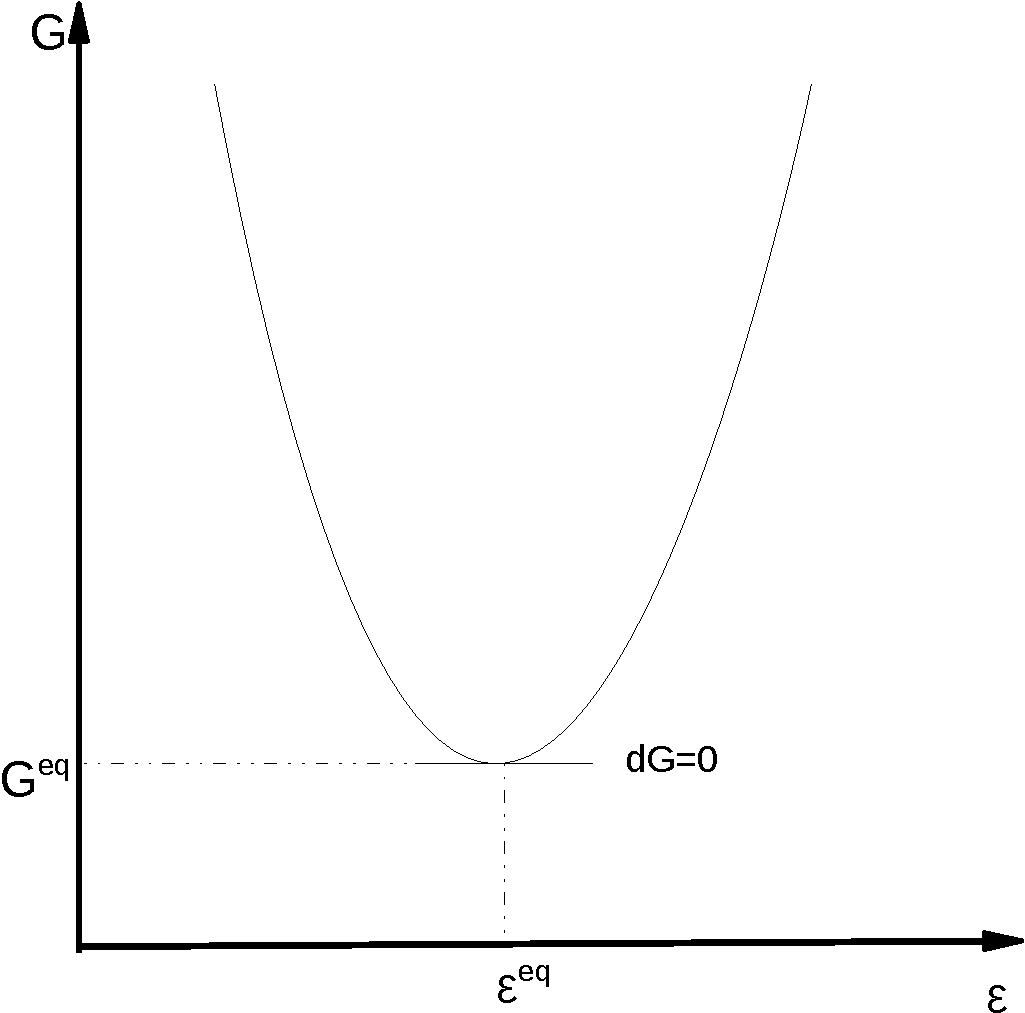
\includegraphics[width=0.5\columnwidth,clip]{./Figs/Mod06_SchematicEquilibriumGibbs_b}
           \caption{Sketch of equilibrium Gibbs free energy.}\label{Chapter:ChemicalReactions:Fig:Fig02}
         \end{center}
      \end{figure} 
   Differentiating Eqn.~\ref{Chapter:ChemicalReactions:Eqn:4a} \wrt $\varepsilon$,
       \begin{displaymath}
           \frc{dG^{t}}{d\varepsilon} = \cancelto{0}{\frc{d}{d\varepsilon}\summation[n_{i,0}\overline{G}_{i}]{i}{}} + \frc{d}{d\varepsilon}\left[\summation[\left(\nu_{i}\varepsilon\right)\overline{G}_{i}]{i}{}\right] = 0,
       \end{displaymath}
   where the summation in brackets can be simplified as,
       \begin{displaymath}
           \frc{d}{d\varepsilon}\left(\nu_{i}\varepsilon \overline{G}_{i}\right) = \nu_{i}G_{i}\cancelto{1}{\frc{d\varepsilon}{d\varepsilon}} + \nu_{i}\varepsilon\cancelto{0}{\frc{d \overline{G}_{i}}{d\varepsilon}} = \nu_{i}\overline{G}_{i}
       \end{displaymath} 
   with $\nu_{i}$ constant, leading to
        \begin{shaded}
          \begin{equation}
             \summation[\nu_{i}\overline{G}_{i}]{i}{} = 0 = \summation[\nu_{i}\mu_{i}]{i}{}.\label{Chapter:ChemicalReactions:Eqn:4b}
          \end{equation}
        \end{shaded}
\end{subequations}


%%% SECTION
\section{Equilibrium Constant of Reactions}\label{Chapter:ChemicalReactions:Section:EquilibriumConstantReactions}\index{Chemical reaction!Equilibrium constant}\index{Equilibrium constant|see{Chemical reaction}}
\begin{subequations}

   The chemical potential was previously defined for mixtures (see Eqn.~\ref{Chapter:SolutionThermodynamics:Eqn:fugacity1b}) as,
       \begin{displaymath}
           \mu_{i} = \Partial[\left(nG\right)]{n_{i}}{T,P,n_{j\ne i}} = \overline{G}_{i} = RT\ln{\overline{f}_{i}} + C_{i}(T),
       \end{displaymath}
   where $\overline{f}_{i}$ is the fugacity of component $i$ in the mixture\footnote{In Chapter~\ref{Chapter:SolutionThermodynamics}, we have studied forms to calculate $\mfr[\overline{f}]{i}{j}$:
      \begin{enumerate}[a)]
          \item ideal gases: $\mfr[\overline{f}]{i}{\text{ig}} =  y_{i}P=P_{i}$ (Dalton law);
          \item real gases: $\mfr[\overline{\phi}]{i}{V}  = \frc{\mfr[\overline{f}]{i}{V}}{y_{i}P}$;
          \item ideal solution: $\mfr[\overline{f}]{i}{\text{id}} = x_{i}\mfr[f]{i}{L}$ (Lewis-Randall rule);
          \item real solution: $\mfr[\overline{f}]{i}{L} = x_{i}\gamma_{i}\mfr[f]{i}{L}$.
      \end{enumerate}
}. At {\it standard state} (\ie pure component at 1 atm), the partial molar Gibbs free energy
      \begin{displaymath}
            \overline{G}_{i}^{\circ}\left(T,P=1\text{ atm}, x_{i}^{\circ}\right) = RT\ln{\overline{f}_{i}^{\circ}} + C_{i}(T),
      \end{displaymath}
      where $x_{i}^{\circ}$ is usually assumed to be either composition of the pure component $\left(\text{\ie }x_{i}^{\circ}=1\right)$, or infinite dilution state $\left(\text{\ie }x_{i}^{\circ}=0\right)$ or ideal 1 molal solution, depending on the nature of the species\footnote{For simplicity of the notation, in this section, $x_{i}$ will represent the mole fraction of species in liquid and vapour phases.}.  $\overline{f}_{i}^{\circ}$ is the fugacity of component $i$ in the mixture at standard conditions. Subtracting the equation above from the previous one, results in,
      \begin{equation}
         \overline{G}\left(T,P, x_{i}\right)  - \overline{G}_{i}^{\circ}\left(T,P=1\text{ atm}, x_{i}^{\circ}\right) = RT\ln{\frc{\overline{f}_{i}}{\overline{f}_{i}^{\circ}}}.\label{Chapter:ChemicalReactions:Eqn:5a}
      \end{equation}
      The log-term was previously (Eqn.~\ref{Chapter:SolutionThermodynamics:Eqn:activity1b}) defined as the activity, \ie $a_{i} = \frc{\overline{f}_{i}}{\overline{f}_{i}^{\circ}}$, and if Eqn.~\ref{Chapter:ChemicalReactions:Eqn:5a} is substituted in Eqn.~\ref{Chapter:ChemicalReactions:Eqn:4b},
      \begin{displaymath}
         0 = \summation[\nu_{i}\overline{G}_{i}]{i}{} = \underbrace{\summation[\nu_{i}\overline{G}_{i}^{\circ}]{i}{}}_{\Delta G_{r}^{\circ}} + RT\summation[\nu_{i}\ln{a_{i}}]{i}{}
      \end{displaymath}
      where $\Delta G_{r}^{\circ} = \summation[\nu_{i}\overline{G}_{i}^{\circ}\left(T,P=1\text{ atm}, x_{i}^{\circ}\right)]{i}{}$ is the Gibbs energy change on reaction with each species (reactants and products) in its standard state or state of unity activity. Using logarithm properties, we can simplify this expression and introduce the {\it product}, $\prod$,\footnote{See Appendix~\ref{Chapter:LogExpReview:Section:Log} for log-properties. In summary, for a set of reals $a_{i}$, $b_{i}$ and $n_{i}$ $\forall i\in\left\{1,2,\cdots, z\right\}$, with $b_{i}\ne 0$,
         \begin{eqnarray}
           \summation[n_{i}\ln{\frc{a_{i}}{b_{i}}}]{i=1}{z} =  \summation[\ln{\left(\frc{a_{i}}{b_{i}}\right)^{n_{i}}}]{i=1}{z} &=& \ln{\left(\frc{a_{1}}{b_{1}}\right)^{n_{1}}} + \ln{\left(\frc{a_{2}}{b_{2}}\right)^{n_{2}}}  + \ln{\left(\frc{a_{3}}{b_{3}}\right)^{n_{3}}} + \cdots + \ln{\left(\frc{a_{z}}{b_{z}}\right)^{n_{z}}} \nonumber \\
                                                                                 &=& \ln{\left[\left(\frc{a_{1}}{b_{1}}\right)^{n_{1}} \cdot \left(\frc{a_{2}}{b_{2}}\right)^{n_{2}} \cdot \left(\frc{a_{3}}{b_{3}}\right)^{n_{3}} \cdots \left(\frc{a_{z}}{b_{z}}\right)^{n_{z}} \right]}  \nonumber \\
                                                                                 &=& \ln{\left[\prod\limits_{i=1}^{z} \left(\frc{a_{i}}{b_{i}}\right)^{n_{i}}\right]}  \nonumber
                    \end{eqnarray}
}
      \begin{shaded}
         \begin{displaymath}
             \ln{\prod\limits_{i=1}^{\mathcal{C}} a_{i}^{\nu_{i}}} = - \frc{\Delta G_{r}^{\circ}}{RT} \;\;\;\;\;\; \Longleftrightarrow \;\;\;\;\; \prod\limits_{i=1}^{\mathcal{C}} a_{i}^{\nu_{i}} = \underbrace{\exp{\left[- \frc{\Delta G_{r}^{\circ}}{RT}\right]}}_{K},
         \end{displaymath}
         \blue{$K$} is the \blue{\it equilibrium constant} and is a function of the system temperature, \ie $K=K(T)$,
         \begin{equation}
             K(T) = \exp{\left[- \frc{\Delta G_{r}^{\circ}}{RT}\right]} = \prod\limits_{i=1}^{\mathcal{C}} a_{i}^{\nu_{i}}. \label{Chapter:ChemicalReactions:Eqn:5b}
         \end{equation}
         The equilibrium constant is independent of the system's composition and pressure but is dependent on the temperature and the reference pressure. The larger the equilibrium constant $\left(\text{which corresponds to more negative values of } \Delta G_{r}^{\circ}\right)$, the further the reaction proceeds to completion. If the standard state of each chemical species in the reaction is chosen to be $T=298.15$ K and $P= 1$ atm,
         \begin{displaymath}
              \Delta G_{r}^{\circ} \left(T=298.15\text{ K}\right) = \summation[\nu_{i}\Delta G_{i,f}^{\circ}\left(T=298.15\text{ K}\right)]{i}{},
         \end{displaymath}
         where $\Delta G_{i,f}^{\circ}$ is the standard state Gibbs free energy of formation, briefly discussed in Section~\ref{Chapter:ChemicalReactions:Section:EnthalpyGibbsReaction}.
      \end{shaded}


%%% SUBSECTION
\subsection{Dependence of $K$ with Temperature}\label{Chapter:ChemicalReactions:Section:K_Temperature}\index{Chemical reaction!Van't Hoff equation}\index{Van't Hoff equation|see{Chemical reaction}}\index{Endothermic reactions}\index{Exothermic reactions}\index{Chemical reaction!Equilibrium constant}\index{Enthalpy! of reaction}
      The equilibrium constant $K$ is strongly dependent on the system temperature, and therefore it is important to be able to define it at any reaction conditions. The {\it Van't Hoff} equation provides a way to correlate $K$ and the enthalpy of reaction $\left(\Delta H^{\circ}_{r}\right)$, using Eqn.~\ref{Chapter:ThermodynamicPropertiesPureFluids:Eqn:GibbsGeneratingFunctionPConst} (for constant pressure conditions) at standard state, 
      \begin{displaymath}
          \overline{H}_{i}^{\circ} = -RT^{2}\frc{d}{dT}\left(\overline{G}_{i}^{\circ}/RT\right) \;\;\;\;\Longrightarrow\;\;\;\;\; \Delta H^{\circ}_{r} = -RT^{2}\frc{d}{dT}\left(\Delta G^{\circ}_{r}/RT\right),
      \end{displaymath}
      where $\Delta H^{\circ}_{r}$ is the standard heat (or enthalpy) of reaction. 
  
      \begin{shaded}
      \noindent Replacing Eqn.~\ref{Chapter:ChemicalReactions:Eqn:5b} in the relation above leads to the \blue{\it Van't Hoff equation},
      \begin{equation}
         \frc{d}{dT}\left(\Delta G^{\circ}_{r}/RT\right) = -\frc{d\left(\ln{K}\right)}{dT} = -\frc{\Delta H^{\circ}_{r}}{RT^{2}}\label{Chapter:ChemicalReactions:Eqn:5c}
      \end{equation}
      \end{shaded}

      \noindent The Van't Hoff equation can be integrated between two temperature levels,
      \begin{displaymath}
           \int\limits_{K_{1}}^{K_{2}}d\left(\ln{K}\right) = \int\limits_{T_{1}}^{T_{2}}\frc{\Delta H^{\circ}}{RT^{2}} dT \;\;\;\Longrightarrow \;\;\; \left(\ln{K_{2}}-\ln{K_{1}}\right) = -\frc{\Delta H^{\circ}}{R}\left(\frc{1}{T_{2}}-\frc{1}{T_{1}}\right).
      \end{displaymath}
      For a qualitative analysis, we can plot $\ln{K} \times 1/T$, and the slope of the linear equation $\left(\text{\ie } y=ax+b,\text{ where }\right.$ $\left.y=\ln{K}\text{ and }x=\frac{1}{T}\right)$ is $-\Delta H^{\circ}/R$. Let's consider reactions for formation of carbon and nitrogen monoxides,
         \reaction[chemreaction:FormationCOb]{C + \frac{1}{2}O_{2} <=> CO}
         \reaction[chemreaction:FormationNO]{\frac{1}{2}N_{2} + \frac{1}{2}O_{2} <=> NO}
      with $\ln{K} \times 1/T$ plot for these reactions in Fig.~\ref{Chapter:ChemicalReactions:Fig:Fig03}. We can qualitatively analyse the behaviour of the equilibrium constant at 1666.67 K and 833.33 K,
      \begin{figure}[hpt] 
         \begin{center}
           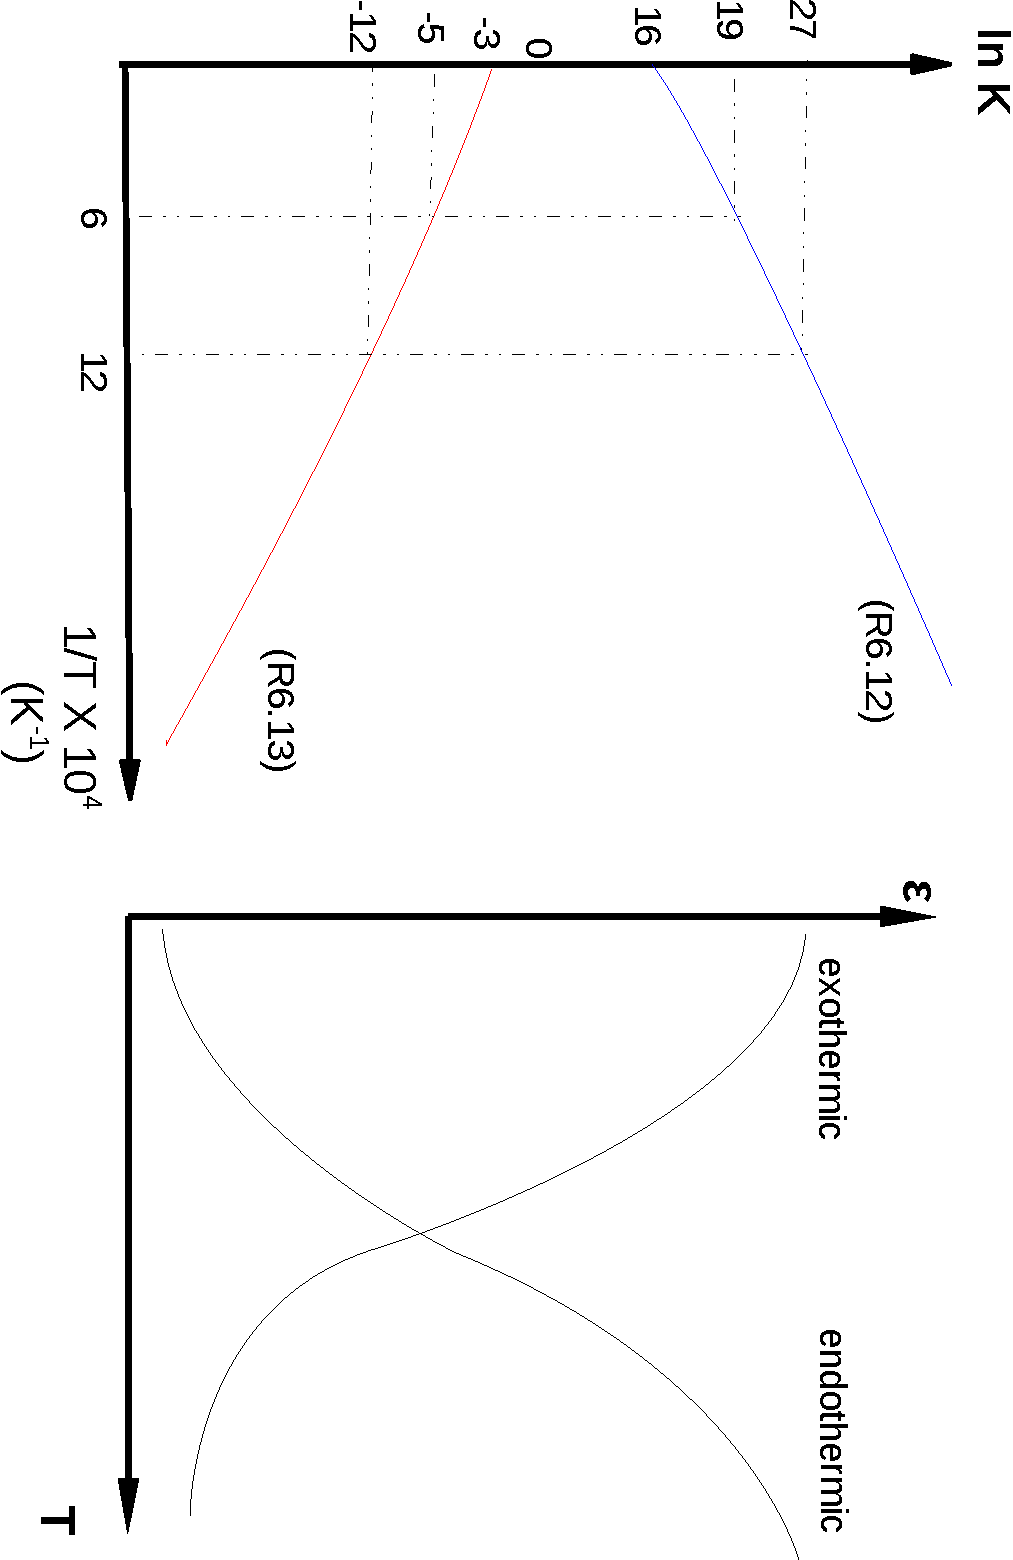
\includegraphics[width=0.5\columnwidth,angle=90,clip]{./Figs/Mod06_SchematicVantHoff_b}
           \caption{(Left) Sketch of equilibrium constants as a function of temperature for reactions~\ref{chemreaction:FormationCOb} and~\ref{chemreaction:FormationNO} \citep[data extracted from][]{SmithVanNess_Book}. (Right) Reaction coordinate $\times$ temperature -- qualitative analysis for endothermic/exothermic reactions based on the standard heat of reaction.}\label{Chapter:ChemicalReactions:Fig:Fig03}
         \end{center}
      \end{figure} 
     
      \begin{displaymath}
        \begin{cases}
            -\left[\frc{\Delta H^{\circ}}{R}\right]_{\ref{chemreaction:FormationCO}} =  \frc{27 - 19}{12-6} = 1.3333, &  \\
            -\left[\frc{\Delta H^{\circ}}{R}\right]_{\ref{chemreaction:FormationNO}} =  \frc{-12 - (-5)}{12-6} = -1.1667 &
          \end{cases}
      \end{displaymath}
      Reactions that present positive $\Delta H^{\circ}$ (\ie negative slope) are called {\it endothermic}, \ie equilibrium constant rises as the temperature is increased (or in other words, heat is given to the reactive system to promote the reaction). Similarly, negative $\Delta H^{\circ}$ (\ie positive slope) are called {\it exothermic}, \ie an increase in temperature leads to a decrease in the equilibrium constant (heat is transferred from the reactive system to the surroundings).

\begin{comment}
%%% SUBSECTION
\subsection{Dependence of $K$ with Temperature}\label{Chapter:ChemicalReactions:Section:K_Temperature}
%\begin{subequations}
    The fundamental thermodynamic relation for the Gibbs free energy at stadard state conditions,
       \begin{displaymath}
           G_{i}^{\circ} = H_{i}^{\circ} - TS_{i}^{\circ},
       \end{displaymath}
   can be extended to chemical reactions at standard state conditions (using Eqn.~\ref{Chapter:ChemicalReactions:Eqn:3b})
       \begin{equation}
           \underbrace{\summation[\nu_{i}G_{i}^{\circ}]{}{}}_{\Delta G^{\circ}} =  \underbrace{\summation[\nu_{i}H_{i}^{\circ}]{}{}}_{\Delta H^{\circ}} - T \underbrace{\summation[\nu_{i}S_{i}^{\circ}]{}{}}_{\Delta S^{\circ}},\label{Chapter:ChemicalReactions:Eqn:6a}
       \end{equation}
   where,
   \begin{enumerate}[i)]
       \item standard heat (enthalpy) of reaction $\left(\Delta H^{\circ}\right)$: starting from the definition of heat capacity at constant pressure, $C_{p}=\Partial[H]{T}{P}$, at standard conditions,
            \begin{eqnarray}
                 && dH_{i}^{\circ} = C_{p_{i}}^{\circ} dT \hspace{4cm}\blue{\left(\times \summation[\nu_{i}]{}{}\right)} \nonumber \\
                 && \summation[\nu_{i}dH_{i}^{\circ}]{}{} = \summation[\nu_{i}C_{p_{i}}^{\circ} dT]{}{} \nonumber \\
                 && \summation[d\left(\nu_{i}H_{i}^{\circ}\right)]{}{} = d\underbrace{\summation[\nu_{i}H_{i}^{\circ}]{}{}}_{\Delta H^{\circ}} = \underbrace{\summation[\nu_{i}C_{p_{i}}^{\circ}]{}{}}_{\Delta C_{p}^{\circ}}dT \nonumber \\
                 && \int d\left(\Delta H^{\circ}\right) = \int \Delta C_{p}^{\circ} dT \nonumber \\
                 && \Delta H^{\circ} - \Delta H^{\circ}_{0} = \blue{R}\int\limits_{T_{0}}^{T} \frc{\Delta C_{p}^{\circ}}{\blue{R}} dT \nonumber
            \end{eqnarray}
            here $R$ is acting as an {\it artifact} that will vanish in a later stage.

       \item standard entropy of reaction $\left(\Delta S^{\circ}\right)$: from the relation $\Partial[S]{T}{P}=\frc{C_{p}}{T}$,
            \begin{eqnarray}
                 && dS_{i}^{\circ} = C_{p_{i}}^{\circ} \frc{dT}{T} \nonumber \\
                 && \int d\left(\Delta S^{\circ}\right) = \int\limits_{T_{0}}^{T}\Delta C_{p}^{\circ}\frc{dT}{T} \nonumber \\
                 && \Delta S^{\circ} - \Delta S^{\circ}_{0} = \blue{R}\int\limits_{T_{0}}^{T}\frc{\Delta C_{p}^{\circ}}{\blue{R}} \frc{dT}{T} \nonumber 
            \end{eqnarray}
   \end{enumerate}
  Replacing these two terms in Eqn.~\ref{Chapter:ChemicalReactions:Eqn:6a} to obtain $\Delta G^{\circ}$
     \begin{eqnarray}
         \Delta G^{\circ} &=&  \Delta H^{\circ}_{0} + \blue{R}\int\limits_{T_{0}}^{T} \frc{\Delta C_{p}^{\circ}}{\blue{R}} dT - T\overbrace{\Delta S^{\circ}_{0}}^{\frc{\Delta H^{\circ}_{0}-\Delta G^{\circ}_{0}}{T_{0}}} - \blue{R}T\int\limits_{T_{0}}^{T}\frc{\Delta C_{p}^{\circ}}{\blue{R}} \frc{dT}{T} \;\;\;\;\; \blue{\times\left(\frc{1}{RT}\right)} \nonumber \\ 
         \underbrace{\frc{\Delta G^{\circ}}{RT}}_{-\ln{K}} &=&  \frc{\Delta G^{\circ}_{0}-\Delta H^{\circ}_{0}}{RT_{0}} + \frc{\Delta H^{\circ}_{0}}{RT} + \frc{1}{T}\int\limits_{T_{0}}^{T} \frc{\Delta C_{p}^{\circ}}{R}dT - \int\limits_{T_{0}}^{T}\frc{\Delta C_{p}^{\circ}}{R}dT \label{Chapter:ChemicalReactions:Eqn:6b}
     \end{eqnarray}
  The standard heat capacities, $\Delta C_{p}^{\circ}=\summation[\nu_{i}C_{p_{i}}^{\circ}]{}{}$ are often expressed as polynomials of the temperature for a range of chemical species. This ensures a sensitivity of this thermophysical parameter with respect to the temperature. In such cases, Eqn.~\ref{Chapter:ChemicalReactions:Eqn:6b} can only be solved numerically with the integrals ranging from the standard (or reference) temperature, $T_{0}$, to $T$. In addition, $\Delta G^{\circ}_{0}$ and $\Delta H^{\circ}_{0}$, Gibbs free energy and enthalpy of reaction at standard pressure conditions (\ie 1 atm) and at reference (or standad) temperature conditions (\ie 298.15 K) are tabulated and readily available in the literature for a number of (relatively) simple chemical reactions.

%\end{subequations}
\end{comment}

%%% SUBSECTION
\subsection{Dependence of $K$ with Composition}\label{Chapter:ChemicalReactions:Section:K_Composition}\index{Fugacity}\index{Fugacity! Coefficient}\index{Solutions!Activity coefficient}
    Recall that in Eqn.~\ref{Chapter:ChemicalReactions:Eqn:5b}, the equilibrium constant $K$ was defined as function of the activities of the reactive mixture,
    \begin{displaymath}
       K = \prod\limits_{i=1}^{\mathcal{C}} a_{i}^{\nu_{i}} = \prod\limits_{i=1}^{\mathcal{C}} \left(\frc{\overline{f}_{i}}{\overline{f}_{i}^{\circ}}\right)^{\nu_{i}}.
    \end{displaymath}
    As the standard state of a gas is the ideal gas state at $P^{\circ}=1\text{ atm}$, the fugacity of an ideal gas in the standard state is equal to its pressure $\overline{f}_{i}^{\circ}=P^{\circ}$ for each reactive species $i$, thus
    \begin{displaymath}
       K = \prod\limits_{i=1}^{\mathcal{C}} \left(\frc{\overline{f}_{i}}{P^{\circ}}\right)^{\nu_{i}},
    \end{displaymath}
    however, for the gaseous phase $\overline{f}_{i} = \overline{\phi}_{i}y_{i}P$,
    \begin{displaymath}
        K = \prod\limits_{i=1}^{\mathcal{C}} \left(\frc{\overline{\phi}_{i}y_{i}P}{P^{\circ}}\right)^{\nu_{i}} = \left[\prod\limits_{i=1}^{\mathcal{C}} \left(\overline{\phi}_{i}y_{i}\right)^{\nu_{i}}\right]\left(\frc{P}{P^{\circ}}\right)^{\summation[\nu_{i}]{i}{} }.
    \end{displaymath}
    \begin{shaded}    
       \noindent Defining $\nu=\summation[\nu_{i}]{i}{}$,
       \begin{equation}
           \prod\limits_{i=1}^{\mathcal{C}} \left(\overline{\phi}_{i}y_{i}\right)^{\nu_{i}} = K\left(\frc{P}{P^{\circ}}\right)^{-\nu}\;\;\;\;\blue{\text{ (for gaseous phase).}}\label{Chapter:ChemicalReactions:Eqn:5d}
       \end{equation}
       At low pressure or high temperature, the fluid behaves as an ideal gas, \ie $\overline{\phi}_{i}=1$, thus
       \begin{equation}
           \prod\limits_{i=1}^{\mathcal{C}} y_{i}^{\nu_{i}} = K\left(\frc{P}{P^{\circ}}\right)^{-\nu}\;\;\;\;\blue{\text{ (for ideal gases).}}\label{Chapter:ChemicalReactions:Eqn:5e}
       \end{equation}
    \end{shaded}
    Now, for the liquid phase the expression previously defined 
    \begin{displaymath}
       K = \prod\limits_{i=1}^{\mathcal{C}} \left(\frc{\overline{f}_{i}}{\overline{f}_{i}^{\circ}}\right)^{\nu_{i}},
    \end{displaymath}
    still holds, and for {\it pure liquid} $i$ at $T$ and 1 atm, using $\overline{f}_{i} = \gamma_{i}x_{i}f_{i}$ (Eqn.~\ref{Chapter:SolutionThermodynamics:Eqn:activity1g}), where $f_{i}$ is the fugacity of pure component $i$ in the liquid phase at $P$ and $T$. Hence,
    \begin{displaymath}
       \frc{\overline{f}_{i}}{\overline{f}_{i}^{\circ}} = \frc{\gamma_{i}x_{i}f_{i}}{\overline{f}_{i}^{\circ}} = \gamma_{i}x_{i}\left(\frc{f_{i}}{\overline{f}_{i}^{\circ}}\right).
    \end{displaymath}
    The fugacity ratio in brackets can be obtained by manipulating the Maxwell relation, $\Partial[G]{P}{T}=V$, and integrating from standard state to $T$ and $P$,
    \begin{eqnarray}
          G_{i}-G_{i}^{\circ} &=& \int\limits_{P^{\circ}}^{P}V_{i}dP \nonumber  \\
          RT\ln{\left(\frc{f_{i}}{f_{i}^{\circ}}\right)} &=& \int\limits_{P^{\circ}}^{P}V_{i}dP \;\;\;\Longrightarrow\;\;\; \ln{\left(\frc{f_{i}}{f_{i}^{\circ}}\right)} = \frc{V_{i}\left(P-P^{\circ}\right)}{RT}, \nonumber
    \end{eqnarray}
    assuming that fluids at liquid phase are incompressible $\left(\text{\ie } V_{i} \text{ is constant}\right)$. Now, replacing in the original equation\footnote{Here, properties of exponents (see Appendix~\ref{Chapter:LogExpReview:Section:Exp}) are used to operate over the thermodynamic properties. Given the set of reals $a_{i}$ and $b_{i}$ $\forall i\in\left\{1,2,\cdots, z\right\}$ and constants $c$ and $d$:
   \begin{enumerate}[a)]
       \item $\left(e^{c}\right)^{d} = e^{cd}$;
       \item $e^{a_{1}b_{1}c}\cdot e^{a_{2}b_{2}c}\cdots e^{a_{z}b_{z}c} = e^{c\left(a_{1}b_{1}+a_{2}b_{2}+\cdots+a_{z}b_{z}\right)}$.
   \end{enumerate}
},
    \begin{eqnarray}
          K &=& \prod\limits_{i=1}^{\mathcal{C}} \left(\frc{\overline{f}_{i}}{\overline{f}_{i}^{\circ}}\right)^{\nu_{i}} = \prod\limits_{i=1}^{\mathcal{C}} \left[\gamma_{i}x_{i}\left(\frc{f_{i}}{\overline{f}_{i}^{\circ}}\right)\right]^{\nu_{i}} \nonumber \\
            &=& \prod\limits_{i=1}^{\mathcal{C}} \left[\gamma_{i}x_{i}\exp{\left(\frc{V_{i}\left(P-P^{\circ}\right)}{RT}\right)}\right]^{\nu_{i}}  = \prod\limits_{i=1}^{\mathcal{C}}\left(\gamma_{i}x_{i}\right)^{\nu_{i}} \times \left\{\exp{\left[\summation[\frc{V_{i}\left(P-P^{\circ}\right)}{RT}]{i}{}\right]}\right\}^{\nu_{i}} \nonumber \\
            &=& \prod\limits_{i=1}^{\mathcal{C}}\left(\gamma_{i}x_{i}\right)^{\nu_{i}} \times \exp{\left[\frc{P-P^{\circ}}{RT}\summation[V_{i}\nu_{i}]{i=1}{\mathcal{C}}\right]}\nonumber
    \end{eqnarray}
    \begin{shaded}
       \begin{equation}
           \prod\limits_{i=1}^{\mathcal{C}}\left(\gamma_{i}x_{i}\right)^{\nu_{i}} = K\exp{\left[\frc{P^{\circ}-P}{RT}\summation[V_{i}\nu_{i}]{i=1}{\mathcal{C}}\right]}\;\;\;\;\blue{\text{ (for liquid phase).}}\label{Chapter:ChemicalReactions:Eqn:5f}
       \end{equation}
       Simplifications:
       \begin{enumerate}[a)]
           \item At room pressure conditions, $P^{\circ}-P=0$ and
              \begin{equation}
                 K = \prod\limits_{i=1}^{\mathcal{C}}\left(\gamma_{i}x_{i}\right)^{\nu_{i}} \;\;\;\;\blue{\text{ (for liquid phase at room pressure conditions).}}\label{Chapter:ChemicalReactions:Eqn:5g}
              \end{equation}
              Although at first sight this equation may seem relatively simple to solve, activity coefficient models are often necessary to be used making it complex to solve, in such cases iterative methods are commonly employed;
           \item For ideal solutions, $\gamma=1$ and Eqn.~\ref{Chapter:ChemicalReactions:Eqn:5g} becomes,
              \begin{equation}
                 K = \prod\limits_{i=1}^{\mathcal{C}}x_{i}^{\nu_{i}} \;\;\;\;\blue{\text{ (for ideal solutions).}}\label{Chapter:ChemicalReactions:Eqn:5h}
              \end{equation}              
       \end{enumerate}
    \end{shaded}
     
\end{subequations}


%%% SECTION
\section{Equilibrium Constant in Multiple Simultaneous Reactions}\label{Chapter:ChemicalReactions:Section:MultipleReactions}
\begin{subequations}
  Calculations of equilibrium constant of single homogeneous chemical reactions can be extended to multiple independent reactions. Let's consider a set of $\mathcal{R}$ independent reactions involving $\mathcal{C}$ chemical species, the equilibrium constant for each reaction is given by an extension of Eqn.~\ref{Chapter:ChemicalReactions:Eqn:5b}
  \begin{shaded}
    \begin{equation}
        K_{j} = \prod\limits_{i=1}^{\mathcal{C}} \left(\frc{\overline{f}_{i}}{\overline{f}_{i}^{\circ}}\right)^{\nu_{i,j}},\;\;\;\;\forall j\in\left\{1,2,\cdots,\mathcal{R}\right\}.\label{Chapter:ChemicalReactions:Eqn:6a}
    \end{equation}
  \end{shaded}
  For {\it gaseous} reactions,
  \begin{shaded}
    \begin{equation}
      K_{j} =
      \begin{cases}
          \prod\limits_{i=1}^{\mathcal{C}} \left(\frc{\overline{f}_{i}}{P^{\circ}}\right)^{\nu_{i,j}},\;\;\;\;\blue{\text{(gas phase),}}\label{Chapter:ChemicalReactions:Eqn:6b} \\
           \\
          \left(\frc{P}{P^{\circ}}\right)^{-\nu_{i,j}}\prod\limits_{i=1}^{\mathcal{C}} \left(y_{i}\right)^{\nu_{i,j}},\;\;\;\;\blue{\text{(ideal gas mixture).}}
      \end{cases}
      \forall j\in\left\{1,2,\cdots,\mathcal{R}\right\}
    \end{equation}
  \end{shaded}



\end{subequations}


\clearpage

%%% SECTION
\section{Examples}

\begin{enumerate}[1)]

%%%
%%% Elliot & Lira (Ex 3.4)  
%%%
\item\label{Example:1} Five moles of hydrogen, two moles of CO and 1.5 moles of CH$_{3}$OH vapour are combined in a batch methanol synthesis reactor (closed system) at 500 K and 1 MPa. Develop expressions for the mole fractions of the species in terms of the reaction coordinate. The components are known to react with the following stoichiometry:
  \begin{displaymath}
      2 H_{2} (g) + CO (g) \Longleftrightarrow CH_{3}OH (g).
  \end{displaymath}

\bigskip

{\bf Solution:} We need to develop expressions for each species in the gaseous form. In the equilibrium, the molar stoichiometric coefficient and the initial number of moles are:
    \begin{displaymath}
       \begin{cases}
         \nu = \sum\limits_{i}\nu_{i}= (-2)+(-1)+(+1)= -2 \;\;\text{ and } \\
         n_{0} = \sum\limits_{i}n_{i,0}= 5 + 2 + 1.5 = 8.5,
       \end{cases}
    \end{displaymath} 
    respectively. Mole fraction of each species is given by
    \begin{displaymath}
          y_{i} = \frc{n_{i}}{n} = \frc{n_{i,0}+\nu_{i}\epsilon}{n_{0}+\nu\epsilon},
    \end{displaymath}
    where the the total number of moles in equilibrium is $n=8.5-2\epsilon$, thus
    \begin{displaymath}
       \begin{cases}
         y_{\text{H}_{2}} = \frc{5-2\epsilon}{8.5-2\epsilon}, \\
         \\
         y_{\text{CO}} = \frc{2-\epsilon}{8.5-2\epsilon}\\
         \\
          y_{\text{CH}_{3}\text{OH}}=\frc{1.5+\epsilon}{8.5-2\epsilon}
       \end{cases}
    \end{displaymath}
\clearpage

\begin{comment}
%%%
%%%   
%%%
\item\label{Example:2} Consider the chemical reaction,
         \begin{displaymath}
             C_{2}H_{4} (g) + H_{2}O (g) \Longleftrightarrow  C_{2}H_{5}OH (g).
         \end{displaymath}
         If an equimolar mixture of ethylene and water vapour is fed to a reactor which is maintained at 500 K and 40 bar, determine the equilibrium constant, assuming that the reaction mixture behaves like an ideal gas. Assume the following ideal gas specific heat data:
         \begin{displaymath}
             C_{p}^{\text{ig}} = a + bT + cT^{2} + dT^{3} + eT^{-2},
         \end{displaymath}
         where C$_{p}^{\text{ig}}$ is expressed in {\it J/mol} and $T$ in $K$. Also,
         \begin{center}
            \begin{tabular}{|c|c c c c c|}
                \hline
                {\it Species}    & $a$    &  $b\times 10^{3}$  & $c\times 10^{6}$ & $d\times 10^{9}$  & $e\times10^{-5}$ \\
                \hline
                C$_{2}$H$_{4}$    & 20.691 &   205.346          & -99.793         & 18.825           & --               \\
                H$_{2}$O         & 4.196  &  154.565           & -81.076         &  16.813          & --               \\
                C$_{2}$H$_{5}$OH  & 28.850 &  12.055            & --              &  --              & 1.006           \\
                \hline
            \end{tabular}
         \end{center}
         The standard state enthalpy and Gibbs energy of reaction are $\Delta H^{0}_{\text{R},298}=-52.7$ kJ/mol and $\Delta G^{0}_{\text{R},298}=14.5$ kJ/mol. In order to calculate the enthalpy of reaction at temperature $T$, $\Delta H^{0}_{T}$, you should use,
         \begin{displaymath}
            \Delta H^{0}_{T} = \Delta H^{0}_{\text{R},298} + \int\limits_{T_{0}}^{T} \Delta C_{p} dT = \Delta H^{0}_{\text{R},298} + \int\limits_{T_{0}}^{T}\left(\Delta a + \Delta bT + \Delta cT^{2} + \Delta dT^{3} + \Delta eT^{-2}\right) dT
         \end{displaymath} 
         where $\Delta a= \sum\limits_{i} \nu_{i}a_{i}$, $\Delta b= \sum\limits_{i} \nu_{i}b_{i}$, $\Delta c= \sum\limits_{i} \nu_{i}c_{i}$, $\Delta d= \sum\limits_{i} \nu_{i}d_{i}$ and $\Delta e= \sum\limits_{i} \nu_{i}e_{i}$.  Also, given the Van't Hoff equation:
         \begin{displaymath}
            \frc{d}{dT}\left(\Delta G^{0}/RT\right) = -\frc{\Delta H^{0}}{RT^{2}}.
         \end{displaymath}


\bigskip

{\bf Solution:}

   \begin{itemize}
      \item We first need to obtain the integral expression for the heat of reaction at temperature $T$,
         \begin{displaymath}
            \Delta H^{0}_{T} = \Delta H^{0}_{\text{R},298} + \int\limits_{T_{0}}^{T} \Delta C_{p} dT = \Delta H^{0}_{\text{R},298} + \int\limits_{T_{0}}^{T}\left(\Delta a + \Delta bT + \Delta cT^{2} + \Delta dT^{3} + \Delta eT^{-2}\right) dT
         \end{displaymath} 
         with 
         \begin{center}
             \begin{tabular}{r l c}
                $\Delta a =$ & $(+1).(28.850)-\left[(-1).(20.691)+(-1).(4.196)\right]=$ & 3.963 \\
                $\Delta b =$ & $\left\{(+1).(12.055)- \left[(-1).(205.346)+(-1).(154.565)\right]\right\}\times 10^{-3}=$ & 0.37197 \\
                $\Delta c =$ & $\left\{(+1).(0)-\left[(-1).(-99.793)+(-1).(-81.076)\right]\right\}\times 10^{-6}=$       & -1.8087$\times$10$^{-4}$  \\
                $\Delta d =$ & $\left\{(+1).(0)-\left[(-1).(18.825)+(-1).(16.813)\right]\right\}\times 10^{-9}=$         & 3.5638$\times$10$^{-8}$\\
                $\Delta e =$ & $\left\{(+1).(1.006)-\left[(-1).(0)+(-1).(0)\right]\right\}\times 10^{5}=$                & 1.006$\times$10$^{5}$ \\
             \end{tabular}
         \end{center}
         Thus,
         \begin{eqnarray}
            \Delta H^{0}_{T} &=& \Delta H^{0}_{\text{R},298} + \int\limits_{T_{0}}^{T} \Delta C_{p} dT = \Delta H^{0}_{\text{R},298} + \int\limits_{T_{0}}^{T}\left(\Delta a + \Delta bT + \Delta cT^{2} + \Delta dT^{3} + \Delta eT^{-2}\right) dT \nonumber \\
            &=& -52.7 + \int\limits_{T_{0}}^{T} \left(3.963 + 0.37197 T - 1.8087\times 10^{-4} T^{2} + 3.5638\times 10^{-8} T^{3} + \frc{1.006 \times 10^{5}}{T^{-2}} \right)dT \nonumber
         \end{eqnarray}
%
      \item We can calculate the Gibbs energy of the reaction through the Van't Hoff equation:
         \begin{displaymath}
                \frc{d}{dT}\left(\Delta G^{0}/RT\right) = -\frc{\Delta H^{0}}{RT^{2}}.
         \end{displaymath}
         Integrating this equation from the standard state temperature, 298.15 K, to $T=$ 500 K

          
   \end{itemize}
\clearpage
\end{comment}

%%%
%%%   Nguyen (Ex 6.6.1)  
%%%
\item\label{Example:2} Ethylene is produced from the decomposition of ethane,
       \begin{displaymath}
          C_{2}H_{6} (g) \Longleftrightarrow C_{2}H_{4} (g) + H_{2} (g) 
       \end{displaymath} 
       Determine the equilibrium composition at 1000$^{\circ}$C and 1 atm. Assume that, initially, there is 1 mol of ethane. Given,
       \begin{center}
           \begin{tabular}{|c c c c|}
           \hline
                                        &  C$_{2}$H$_{6}$ (g) & C$_{2}$H$_{4}$ (g) &  H$_{2}$ (g)  \\ 
           \hline
             $\Delta G^{\circ}_{\text{f,298}}$  &  -32.84            &  68.15           & 0.0           \\
                   (kJ/mol)             &                    &                  &               \\
           \hline
             $\Delta H^{\circ}_{\text{f,298}}$  &  -84.68            &  52.26           & 0.0           \\
                   (kJ/mol)             &                    &                  &               \\
           \hline 
           \end{tabular}
       \end{center}
       where $\Delta G^{\circ}_{\text{f,298}}$ and $\Delta H^{\circ}_{\text{f,298}}$ are the standard state Gibbs energy and enthalpy of formation. 

\bigskip

{\bf Solution:} First we need to determine the standard state Gibbs energy of reaction,
         \begin{eqnarray}
             \Delta G^{\circ}_{\text{r,298}} &=& \sum\limits_{i}\nu_{i}\left(\Delta G^{\circ}_{\text{f,298}}\right)_{i} \nonumber \\
                                     &=& (+1).(68.15)+ (1).(0.0) + (-1).(-32.84) = 100.99\; \text{kJ/mol} \nonumber
         \end{eqnarray}
       The equilibrium constant can be obtained from,
         \begin{displaymath}
            K = \exp\left(-\frc{\Delta G^{\circ}_{\text{r,298}}}{RT}\right) = exp\left(-\frc{100.99\times 10^{3}}{(8.314).(298.15)}\right) = 2.0246\times 10^{-18}
         \end{displaymath}
       The Van't Hoff equation can be used to calculate the equilibrium constant at temperature $T$,
         \begin{displaymath}
            \frc{\partial\left(\ln K\right)}{\partial T} = \frc{\Delta H^{\circ}_{\text{r}}}{RT^{2}}
         \end{displaymath}
       Before we can integrate the Van't Hoff equation, we first need to determine the standard heat of reaction, $\Delta H^{\circ}_{\text{r}}$,
         \begin{eqnarray}
            \Delta H^{\circ}_{\text{r}} &=& \sum\limits_{i} \nu_{i}\left(\Delta H^{\circ}_{\text{f,298}}\right)_{i} \nonumber \\
                                 &=& (+1).(52.26) + (+1).(0.0) + (-1).(-84.68) = 136.94\;\text{kJ/mol}\nonumber
         \end{eqnarray}
       Now integrating the Van't Hoff equation from 298.15 K to 1273.15 K,
         \begin{eqnarray}
            \ln\frc{K_{1273}}{K_{298}} &=& -\frc{\Delta H^{\circ}_{\text{r}}}{R}\left(\frc{1}{T}-\frc{1}{298.15}\right) \nonumber \\
            \ln\frc{K_{1273}}{2.0246\times 10^{-18}} &=& -\frc{136.94\times 10^{3}}{8.314}\left(\frc{1}{1273.15}-\frc{1}{298.15}\right) \nonumber \\
            K_{1273} &=& 4.7859 \nonumber
         \end{eqnarray} 
       The equilibrium constant $K$ can also be expressed as a function of the components' activities,
         \begin{displaymath}
            K = \prod\limits_{i=1}^{\mathcal{C}} a_{i}^{\nu_{i}} = \frc{a_{\text{C}_{2}\text{H}_{4}}a_{\text{H}_{2}}}{a_{\text{C}_{2}\text{H}_{6}}} = \frc{\left(\frc{\overline{f}_{\text{C}_{2}\text{H}_{4}}}{\overline{f}^{\circ}_{\text{C}_{2}\text{H}_{4}}}\right)\left(\frc{\overline{f}_{\text{H}_{2}}}{\overline{f}^{\circ}_{\text{H}_{2}}}\right)}{\left(\frc{\overline{f}_{\text{C}_{2}\text{H}_{6}}}{\overline{f}^{\circ}_{\text{C}_{2}\text{H}_{6}}}\right)}
         \end{displaymath}
         Assuming ideal gas behaviour, $\overline{f}_{i}=P_{i}$, $\overline{f}_{i}^{\circ}=P^{\circ}_{\text{C}_{2}\text{H}_{6}}=P^{\circ}_{\text{C}_{2}\text{H}_{4}}=P^{\circ}_{\text{H}_{2}}=$ 1 atm. Thus,
         \begin{displaymath}
            K = \frc{a_{\text{C}_{2}\text{H}_{4}}a_{\text{H}_{2}}}{a_{\text{C}_{2}\text{H}_{6}}} = \frc{\left(\frc{\overline{f}_{\text{C}_{2}\text{H}_{4}}}{\overline{f}^{\circ}_{\text{C}_{2}\text{H}_{4}}}\right)\left(\frc{\overline{f}_{\text{H}_{2}}}{\overline{f}^{\circ}_{\text{H}_{2}}}\right)}{\left(\frc{\overline{f}_{\text{C}_{2}\text{H}_{6}}}{\overline{f}^{\circ}_{\text{C}_{2}\text{H}_{6}}}\right)} = \frc{\left(\frc{P_{\text{C}_{2}\text{H}_{4}}}{P^{\circ}_{\text{C}_{2}\text{H}_{4}}}\right)\left(\frc{P_{\text{H}_{2}}}{P^{\circ}_{\text{H}_{2}}}\right)}{\left(\frc{P_{\text{C}_{2}\text{H}_{6}}}{P^{\circ}_{\text{C}_{2}\text{H}_{6}}}\right)} = \frc{\left(\frc{y_{\text{C}_{2}\text{H}_{4}}P}{1\text{ atm}}\right)\left(\frc{y_{\text{H}_{2}}P}{1\text{ atm}}\right)}{\left(\frc{y_{\text{C}_{2}\text{H}_{6}}P}{1\text{ atm}}\right)}          
         \end{displaymath}
         Since $P=$ 1 atm,
         \begin{displaymath}
            K = \frc{\left(\frc{y_{\text{C}_{2}\text{H}_{4}}P}{1\text{ atm}}\right)\left(\frc{y_{\text{H}_{2}}P}{1\text{ atm}}\right)}{\left(\frc{y_{\text{C}_{2}\text{H}_{6}}P}{1\text{ atm}}\right)} = \frc{\left(y_{\text{C}_{2}\text{H}_{4}}\right)\left(y_{\text{H}_{2}}\right)}{\left(y_{\text{C}_{2}\text{H}_{6}}\right)} = 4.7859
         \end{displaymath}
         This equation can not be solved as there are two unknowns $\left(\text{remember that }\summation[y_{i}]{i=1}{3}=1\right)$. The number of unknowns can be decreased if we make use of
         \begin{displaymath}
           y_{i} = \frc{n_{i}}{n} = \frc{n_{i,0}+\nu_{i}\epsilon}{n_{0}+\nu\epsilon}.
         \end{displaymath}
         with 
         \begin{displaymath}
            \nu = \sum\limits_{i}\nu_{i}= (-1)+(+1)+(+1)= 1 \;\;\text{ and }\;\; n_{0} = \sum\limits_{i}n_{i,0}= 1 + 0 + 0 = 1,
         \end{displaymath} 
       Thus,
         \begin{displaymath}
             y_{\text{C}_{2}\text{H}_{6}} = \frc{1-\epsilon}{1+\epsilon},\;\;y_{\text{C}_{2}\text{H}_{4}} = \frc{\epsilon}{1+\epsilon}\;\text{ and }\;y_{\text{H}_{2}} = \frc{\epsilon}{1+\epsilon}
         \end{displaymath}
       Replacing the compositions in the expression for $K$,
         \begin{eqnarray}
           K  &=& \frc{\left(y_{\text{C}_{2}\text{H}_{4}}\right)\left(y_{\text{H}_{2}}\right)}{\left(y_{\text{C}_{2}\text{H}_{6}}\right)} = \frc{\left(\frc{\epsilon}{1+\epsilon}\right)^{2}}{\left(\frc{1-\epsilon}{1+\epsilon}\right)} =4.7859 \nonumber \\
            &&\epsilon = 0.9095 \nonumber
         \end{eqnarray}
        The equilibrium concentration of C$_{2}$H$_{4}$(g) is $y_{\text{C}_{2}\text{H}_{4}} =$ 0.4763 $=y_{\text{H}_{2}}$ and $y_{\text{C}_{2}\text{H}_{6}}=$ 0.0474.

\clearpage


%%%
%%%   Nguyen (Ex 6.7.2) 
%%%
\item\label{Example:3} Determine the equilibrium conversion for the liquid-phase isomerisation reaction of methylcyclopentane $\left(\text{CH}_{3}\text{C}_{5}\text{H}_{9}\right)$ to cyclohexane $\left(\text{C}_{6}\text{H}_{12}\right)$ at 25$^{\circ}$C. Gibbs energies of formation are given at 25$^{\circ}$C as:
  \begin{displaymath}
     \left(\Delta G^{\circ}_{\text{f,298}}\right)_{\text{CH}_{3}\text{C}_{5}\text{H}_{9}} = 31.72 \text{ kJ.mol}^{-1} \text{ and } \left(\Delta G^{\circ}_{\text{f,298}}\right)_{\text{C}_{6}\text{H}_{12}} = 26.89 \text{ kJ.mol}^{-1}.
  \end{displaymath}
  Also, assume that this isomerisation reaction occurs at relatively low pressure, and therefore $\frc{f_{i}}{f^{\circ}_{i}}=1$. Also, assume that solution is ideal.


\bigskip

{\bf Solution:} The isomerisation reaction can be represented by,
    \begin{displaymath}
        CH_{3}C_{5}H_{9} (l) \Longleftrightarrow C_{6}H_{12} (l)
    \end{displaymath}
    We need to determine the equilibrium constant at room temperature
         \begin{eqnarray}
           \Delta G^{\circ}_{r,298} &=& \sum\limits_{i}\nu_{i}\Delta G^{\circ}_{\text{f,298}} \nonumber \\
                             &=& (+1).\left(\Delta G^{\circ}_{\text{f,298}}\right)_{\text{C}_{6}\text{H}_{12}} + (-1).\left(\Delta G^{\circ}_{\text{f,298}}\right)_{\text{CH}_{3}\text{C}_{5}\text{H}_{9}} \nonumber \\ 
                             &=& 26.89-31.72 = -4.83 \text{ kJ/mol} \nonumber
         \end{eqnarray}
       The equilibrium constant is
         \begin{displaymath}
             K = \exp\left(-\frc{\Delta G^{\circ}_{r,298}}{RT}\right) = \exp\left(-\frc{-4830}{(8.314).(298.15)}\right) = 7.0182
         \end{displaymath}
       The equilibrium constant can also be obtained from 
         \begin{displaymath}
            K = \prod\limits_{i}\left(\frc{\overline{f}_{i}}{\overline{f}^{\circ}_{i}}\right)^{\nu_{i}} = \prod\limits_{i}\left(\frc{x_{i}\gamma_{i} f_{i}}{\overline{f}^{\circ}_{i}}\right)^{\nu_{i}}
         \end{displaymath}
       At room pressure conditions, the ratio $\frc{f_{i}}{\overline{f}^{\circ}_{i}} = \frc{f_{i}}{f_{i}^{\circ}} = \exp\left[\frc{V\left(P-P^{\circ}\right)}{RT}\right]=1$, therefore,
         \begin{displaymath}
            K = \prod\limits_{i}\left(\frc{x_{i}\gamma_{i}f_{i}}{\overline{f}^{\circ}_{i}}\right)^{\nu_{i}} = \prod\limits_{i}\left(x_{i}\gamma_{i}\right)^{\nu_{i}}
         \end{displaymath}
       For ideal solution,
         \begin{displaymath}
            K = \prod\limits_{i=1}^{\mathcal{C}}\left(x_{i}\gamma_{i}\right)^{\nu_{i}} = \prod\limits_{i}\left(x_{i}\right)^{\nu_{i}} = \left(x_{\text{C}_{6}\text{H}_{12}}\right).\left(x_{\text{CH}_{3}\text{C}_{5}\text{H}_{9}}\right)^{-1} = 7.0182,
         \end{displaymath}
         as $\summation[x_{i}]{i}{}=1$, we could easily solve the equation above as $x_{\text{C}_{6}\text{H}_{12}}\left(1-x_{\text{C}_{6}\text{H}_{12}}\right)=7.0182$, and obtain $x_{\text{C}_{6}\text{H}_{12}}=0.8753$. Alternatively, one could obtain a relation between composition and the reaction coordinate, $\varepsilon$,
         \begin{displaymath}
            x_{i} = \frc{n_{i,0} + \nu_{i}\varepsilon}{n_{0}+\nu\epsilon},
         \end{displaymath}
         where $\nu = (-1) + (1) = 0$ and assuming that initially there are $n_{\text{CH}_{3}\text{C}_{5}\text{H}_{9},0}=1$ and $n_{\text{C}_{6}\text{H}_{12},0}=0$,
         \begin{displaymath}
            x_{\text{CH}_{3}\text{C}_{5}\text{H}_{9}} = 1-\varepsilon\;\;\;\;\;\text{ and }\;\;\;\;\;\; x_{\text{C}_{6}\text{H}_{12}} = \varepsilon.
         \end{displaymath}
         Now, replacing in the expression above, 
         \begin{displaymath}
             K = \left(x_{\text{C}_{6}\text{H}_{12}}\right).\left(x_{\text{CH}_{3}\text{C}_{5}\text{H}_{9}}\right)^{-1} = \frc{\varepsilon}{1-\varepsilon} = 7.0182 \;\;\;\; \Longrightarrow \;\;\;\;\; \epsilon = 0.8753 
         \end{displaymath}
         Thus, $x_{\text{C}_{6}\text{H}_{12}}=0.8753$ and $x_{\text{CH}_{3}\text{C}_{5}\text{H}_{9}}=0.1247$.

\clearpage

%%%
%%%  Sandler (Ex 13.1.1, pg. 713)
%%%
\item\label{Example:4} Calculate the equilibrium extent of decomposition of nitrogen tetroxide $\left(N_{2}O_{4}\right)$,
  \begin{displaymath}
     N_{2}O_{4} (g) \Longleftrightarrow 2 NO_{2} (g)
  \end{displaymath}
  at 298.15 K and 1 atm. Assume that the gas mixture behaves as an ideal gas and the Gibbs energies of formation at 25$^{\circ}$C are:
  \begin{displaymath}
     \left(\Delta G^{\circ}_{\text{f,298}}\right)_{N_{2}O_{4}} = 97.89 \text{ kJ.mol}^{-1} \text{ and } \left(\Delta G^{\circ}_{\text{f,298}}\right)_{NO_{2}} = 51.31 \text{ kJ.mol}^{-1}.
  \end{displaymath}
     

\bigskip

{\bf Solution:} 
       The equilibrium constant is
         \begin{displaymath}
             K = \exp\left(-\frc{\Delta G^{\circ}_{r,298}}{RT}\right) = \frc{a_{NO_{2}}^{2}}{a_{N_{2}O_{4}}} = \frc{\left(\frc{y_{NO_{2}}P}{P^{\circ}_{NO_{2}}}\right)^{2}}{\left(\frc{y_{N_{2}O_{4}}P}{P^{\circ}_{N_{2}O_{4}}}\right)} = \frac{\left(y_{NO_{2}}\right)^{2}}{\left(y_{N_{2}O_{4}}\right)},
         \end{displaymath}
         where the standard Gibbs energy of reaction is
         \begin{eqnarray}
           \Delta G^{\circ}_{r,298} &=& \sum\limits_{i}\nu_{i}\Delta G^{\circ}_{\text{f,298}} \nonumber \\
                             &=& (+2).\left(\Delta G^{\circ}_{\text{f,298}}\right)_{NO_{2}} + (-1).\left(\Delta G^{\circ}_{\text{f,298}}\right)_{N_{2}O_{4}} \nonumber \\ 
                             &=& 4730 \text{ J/mol}, \nonumber
         \end{eqnarray}
         and the equilibrium constant,
         \begin{displaymath}
             K = \exp\left(-\frc{\Delta G^{\circ}_{r,298}}{RT}\right) = 0.1484 = \frac{\left(y_{NO_{2}}\right)^{2}}{\left(y_{N_{2}O_{4}}\right)}
         \end{displaymath}
         Composition and reaction coordinate are related through
         \begin{displaymath}
            y_{i} = \frc{n_{i,0} + \nu_{i}\varepsilon}{n_{0}+\nu\epsilon},
         \end{displaymath}
         where, assuming that the initial number of moles are $n_{N_{2}O_{4},0}=1$ and $n_{NO_{2},0}=0$, an $\nu= 2-1 = 1$,
         \begin{displaymath}
            y_{N_{2}O_{4}} = \frc{1-\varepsilon}{1+\varepsilon}\;\;\;\;\;\text{ and }\;\;\;\;\;\; y_{NO_{2}} = \frc{2\varepsilon}{1+\varepsilon},
         \end{displaymath}
         leading to
         \begin{displaymath}
             K = \frac{\left(y_{NO_{2}}\right)^{2}}{\left(y_{N_{2}O_{4}}\right)} = \frc{\left(\frc{2\varepsilon}{1+\varepsilon}\right)^{2}}{\left(\frc{1-\varepsilon}{1+\varepsilon}\right)} = 0.1484 \;\;\;\;\Longrightarrow\;\;\;\; \varepsilon = 0.1891
         \end{displaymath}
         Thus: $y_{NO_{2}} = 0.3181$ and $y_{N_{2}O_{4}} = 0.6819$.

         
\clearpage

%%%
%%%  Sandler (Ex 13.1.2, pg. 714)
%%%
\item\label{Example:5} Pure nitrogen tetroxide $\left(N_{2}O_{4}\right)$ at a low temperature is diluted with nitrogen $\left(N_{2}\right)$ and heated to 298.15 K and 1 atm. If the initial mole fraction of $N_{2}O_{4}$ in the $N_{2}O_{4}-N_{2}$ mixture before the dissociation begins is 0.20, what is the extent of the decomposition, 
  \begin{displaymath}
     N_{2}O_{4} (g) \Longleftrightarrow 2 NO_{2} (g)
  \end{displaymath}
  and the mole fractions of $NO_{2}$ and $N_{2}O_{4}$ present at equilibrium? Assume that the gas mixture behaves as an ideal gas and the Gibbs energies of formation at 25$^{\circ}$C are:
  \begin{displaymath}
     \left(\Delta G^{\circ}_{\text{f,298}}\right)_{N_{2}O_{4}} = 97.89 \text{ kJ.mol}^{-1} \text{ and } \left(\Delta G^{\circ}_{\text{f,298}}\right)_{NO_{2}} = 51.31 \text{ kJ.mol}^{-1}.
  \end{displaymath}

\bigskip

{\bf Solution:} Here, nitrogen is an inert species, \ie it is used to dilute the reactant gas, $N_{2}O_{4}$, but do not participate in the decomposition reaction, thus $\nu_{N_{2}}=0$. In Example~\ref{Example:4}, we have already calculated the equilibrium constant, $K = 0.1484$, and used 
         \begin{displaymath}
            y_{i} = \frc{n_{i,0} + \nu_{i}\varepsilon}{n_{0}+\nu\epsilon},
         \end{displaymath}
         to calculate the equilibrium composition. The overall molar stoichiometric coefficient $\nu= 2-1-0 = 1$ remains the same, however, now the initial reactive composition is (assuming 1 mol of the reactant mixture) $n_{N_{2}O_{4},0} = 0.2$, $n_{N_{2},0} = 0.8$ and $n_{NO_{2},0}=0$. 
         \begin{displaymath}
           y_{N_{2}O_{4}} = \frc{0.2-\varepsilon}{1+\varepsilon},\;\;\;\;\; y_{N_{2}} = \frc{0.8}{1+\varepsilon}\;\;\;\text{ and }\;\;\;y_{NO_{2}} = \frc{2\varepsilon}{1+\varepsilon}.
         \end{displaymath}
         Leading to
         \begin{displaymath}
             K = \frac{\left(y_{NO_{2}}\right)^{2}}{\left(y_{N_{2}O_{4}}\right)} = \frc{\left(\frc{2\varepsilon}{1+\varepsilon}\right)^{2}}{\left(\frc{0.2-\varepsilon}{1+\varepsilon}\right)} = 0.1484 \;\;\;\;\Longrightarrow\;\;\;\; \varepsilon = 0.0715,
         \end{displaymath}
         with equilibrium compositions of $y_{NO_{2}} = 0.1335$, $y_{N_{2}O_{4}} = 0.1199$ and $y_{N_{2}} = 0.7466$. 
         
\clearpage


%%%
%%%  Sandler (Ex 13.1.3, pg. 718)
%%%
\item\label{Example:6} Calculate the equilibrium extent of decomposition of nitrogen tetroxide $\left(N_{2}O_{4}\right)$,
  \begin{displaymath}
     N_{2}O_{4} (g) \Longleftrightarrow 2 NO_{2} (g)
  \end{displaymath}
  at 250 K and 400 K and 1 atm. Assume that the gas mixture behaves as an ideal gas and the Gibbs energies of formation at 25$^{\circ}$C are:
  \begin{displaymath}
     \left(\Delta G^{\circ}_{\text{f,298}}\right)_{N_{2}O_{4}} = 97.89 \text{ kJ.mol}^{-1} \text{ and } \left(\Delta G^{\circ}_{\text{f,298}}\right)_{NO_{2}} = 51.31 \text{ kJ.mol}^{-1}.
  \end{displaymath}
  Also, the standard enthalpy of reaction at 25$^{\circ}$C is 56.189 kJ.mol$^{-1}$. Heat capacity $\left(\text{in J.mol}^{-1}\text{.K}^{-1}\right)$ for both gases are expressed in a polynomial form,
  \begin{displaymath}
    C_{p} = a + bT + CT^{2} + dT^{3},
  \end{displaymath}
  where
  \begin{center}
    \begin{tabular}{ l | c c c c }
      \hline
                         &  $a$     &  $b\times 10^{-2}$  & $c\times 10^{-5}$  & $d\times 10^{-9}$ \\
                         &$\left(\text{J.mol}^{-1}\text{.K}^{-1}\right)$& $\left(\text{J.mol}^{-1}\text{.K}^{-2}\right)$& $\left(\text{J.mol}^{-1}\text{.K}^{-3}\right)$& $\left(\text{J.mol}^{-1}\text{.K}^{-4}\right)$ \\
      \hline
      NO$_{2}$             &  22.929 &      5.711          & -3.519            & 7.866 \\
      N$_{2}$O$_{4}$       &   33.054 &      18.661         &    -11.339        &  -- 
    \end{tabular}
  \end{center}
      

\bigskip

{\bf Solution:} In order to calculate composition at equilibrium, we need to calculate the equilibrium constant, $K$, at 250 K and 400 K through the Van't Hoff equation,
\begin{displaymath}
    \frc{d\left(\ln{K}\right)}{dT} = \frc{\Delta H^{\circ}_{r}}{RT^{2}} \;\;\;\Longrightarrow \;\;\; \ln{\left(\frc{K(T)}{K(298.15\text{ K})}\right)} = \int\limits_{298.15\text{ K}}^{T}\frc{\Delta H^{\circ}_{r}}{RT^{2}}dT.
\end{displaymath}
We have already calculated $K$ at 298.15 in Example~\ref{Example:4}, $K= 0.1484$. The standard heat of reaction is obtained from the fundamental enthalpy relation, $dH= C_{p}dT$, and 
\begin{displaymath}
     \Delta H^{\circ}_{r} = \summation[\nu_{i}\Delta H^{\circ}_{i,f}]{i}{} \;\;\;\Longrightarrow\;\;\; \int\limits_{\Delta H^{\circ}_{r,298.15}}^{\Delta H^{\circ}_{r,T}}d\left(\Delta H^{\circ}_{r}\right) = \int\limits_{298.15\text{ K}}^{T}\summation[\nu_{i} C_{p,i}]{i}{}dT.
\end{displaymath}
The first stage in this calculation is to obtain an expression for the right-hand side integration, \ie the summation term $\Delta C_{p}^{\circ} = \summation[\nu_{i} C_{p,i}]{i}{}$, using (for simplicity in the notation) $NO_{2}$:1 and $N_{2}O_{4}$:2,
\begin{eqnarray}
   \Delta C_{p}^{\circ} &=& \summation[\nu_{i} C_{p,i}]{i}{} = (+2) \left(a_{1}+b_{1}T+c_{1}T^{2}+d_{1}T^{3}\right) + (-1)\left(a_{2}+b_{2}T+c_{2}T^{2}+d_{2}T^{3}\right) \nonumber \\
                     &=& 12.804 - 7.239\times 10^{-2}T + 4.301\times 10^{-5} T^{2} + 15.732\times 10^{-9}T^{3} \nonumber 
\end{eqnarray}
And the integration becomes $\left(\text{with }\Delta H^{\circ}_{r,298.15} = 56189\text{ J.mol}^{-1}\right)$
\begin{eqnarray}
    && \Delta H^{\circ}_{r}(T) - \Delta H^{\circ}_{r,298.15} = \int\Delta C_{p}^{\circ}dT \nonumber \\
    && \Delta H^{\circ}_{r}(T) = 56189 + 12.804 T - \frc{7.239\times 10^{-2}}{2}T^{2} + \frc{4.301\times 10^{-5}}{3}T^{3} + \frc{15.732\times 10^{-9}}{4}T^{4} \nonumber
\end{eqnarray}
Now, using the Van't Hoff equation,
\begin{eqnarray}
  \ln{\left(\frc{K(T)}{K_{298.15\text{ K}}}\right)} &=& \int\limits_{298.15\text{ K}}^{T}\frc{\Delta H^{\circ}_{r}}{RT^{2}}dT \nonumber \\
                                                &=& \frc{1}{R}\int\limits_{298.15\text{ K}}^{T} \left[\frc{56189}{T^{2}} + \frc{12.804}{T} - \frc{7.239\times 10^{-2}}{2} + \frc{4.301\times 10^{-5}}{3}T + \frc{15.732\times 10^{-9}}{4}T^{2}\right]dT \nonumber \\
                                                &=& \frc{1}{R}\left[-\frc{56189}{T} + 12.804\ln{T} - \frc{7.239\times 10^{-2}}{2}T + \frc{4.301\times 10^{-5}}{6}T^{2} + \frc{15.732\times 10^{-9}}{12}T^{3}\right]_{298.15\text{ K}}^{T} \nonumber
\end{eqnarray}
Solving this integral for
\begin{displaymath}
  \begin{cases}
      K_{250\text{ K}} = 1.7298\times 10^{-3} \\
      K_{400\text{ K}} = 51.4338
  \end{cases}  
\end{displaymath}
Now, using the expression obtained in Example~\ref{Example:4} for composition, assuming that the initial number of moles are $n_{N_{2}O_{4},0}=1$ and $n_{NO_{2},0}=0$, and $\nu= 2-1 = 1$,
         \begin{displaymath}
            y_{N_{2}O_{4}} = \frc{1-\varepsilon}{1+\varepsilon}\;\;\;\;\;\text{ and }\;\;\;\;\;\; y_{NO_{2}} = \frc{2\varepsilon}{1+\varepsilon},
         \end{displaymath}
         leading to
         \begin{displaymath}
             K = \frac{\left(y_{NO_{2}}\right)^{2}}{\left(y_{N_{2}O_{4}}\right)} = \frc{\left(\frc{2\varepsilon}{1+\varepsilon}\right)^{2}}{\left(\frc{1-\varepsilon}{1+\varepsilon}\right)}
         \end{displaymath}
         Solving for
         \begin{displaymath}
           \begin{cases}
             K_{250\text{ K}}   = 1.7298\times10^{-3} \;\;\Longrightarrow \varepsilon = 0.02079 \;\;\Longrightarrow \;\; y_{NO_{2}} = 0.0407 \text{ and } y_{N_{2}O_{4}} = 0.9593; \\
             K_{298.15\text{ K}} = 0.1484 \hspace{1.cm} \Longrightarrow  \varepsilon = 0.1891  \hspace{.35cm} \Longrightarrow \;\; y_{NO_{2}} = 0.3181 \text{ and } y_{N_{2}O_{4}} = 0.6819; \\
             K_{400\text{ K}}   = 51.4331 \hspace{1.2cm} \Longrightarrow \varepsilon = 0.9632  \hspace{.35cm} \Longrightarrow \;\;  y_{NO_{2}} = 0.9813 \text{ and } y_{N_{2}O_{4}} = 0.0187 \\
           \end{cases}
         \end{displaymath}
         
        Note that at low temperature, 250 K $\left(-23.15^{\circ}\text{C}\right)$, the production of nitrogen dioxide is fairly small (backward reaction), however as the temperature rises the forward reaction becomes dominant with 98.1$\%$ of NO$_{2}$ being produced at 400 K$\left(126.85^{\circ}\text{C}\right)$.

\end{enumerate}


\clearpage   
\begin{FinalSummaryBlock}{Summary}
     Concepts introduced in this chapter are relatively simple but far reaching. They are cornerstone for the remaining of this notes and for fundamental chemical thermodynamics. An extension of total derivative to multi-component systems led to the equilibrium criteria for general multiphase ($\mathcal{P}\ge2$) and multi-component ($\mathcal{C}\ge2$) mixtures.
    \begin{itemize}
       \item Initial definition and discussion of excess properties (Eqn.~\ref{Chapter:VLE:Eqn:ExcessProperties1a});
       \item Definition of chemical potential as the partial molar Gibbs free energy (Eqn.~\ref{Chapter:VLE:Eqn:ChemPotentialDef1b}) and development of a fundamental relation for multi-component systems (Eqn.~\ref{Chapter:VLE:Eqn:ChemPotentialDef1d});
       \item Chemical equilibrium can be assessed \wrt thermodynamic conditions as stated in Table~\ref{Chapter:VLE:Table:TableEquilibriumCriteria};
       \item In closed systems at constant pressure and temperature conditions, the criterion for equilibrium is that the Gibbs free energy is the minimum which leads to equality of chemical potential of each component at all phases (Eqn.~\ref{Chapter:VLE:EqnChemPotentialDef1c3});
       \item Multi-component VLE problems (\ie $\mathcal{C}\ge 2$ and $\mathcal{P}=2$) can be represented by $P-T-x_{i}y_{i}$ phase diagrams, where critical pressure and temperature (for individual components and the mixtures), liquid and vapour saturation lines, bubble and dew points can be identified;
       \item Although compositions, temperatures and pressures can be obtained from graphical representation (2-/3-D) of phase equilibrium, this is not very convenient and numerical models were develop to represent the partition of components in both phases in equilibrium;
       \item Raoult's law (Eqn.~\ref{Chapter:VLE:Eqn:RaoultLaw}) is an idealisation of the components' partition between vapour and liquid phases assuming limited molecular forces (\eg attractive and repulsive) act in the liquid phase;
       \item Henry's law (Eqn.~\ref{Chapter:VLE:Eqn:HenryLaw}) is applied to gases solubilised at low concentrations in liquid solutions;
       \item K-value models (Eqn.~\ref{Chapter:VLE:Eqn:KValue}) were mostly developed for petro-chemical industry to help quickly assess concentrations of (light) hydrocarbons in vapour and liquid phases;
       \item Dew and bubble coordinates (pressure, temperature and compositions) in typical industrial applications are discussed in Section~\ref{Chapter:VLE:Section:IndApplications};
       \item Depending on known conditions, four main problems may arise:
\begin{center}
   \begin{tabular}{|l c c|}
      \hline 
      $\mathbf{VLE}$ {\bf Problem} & {\bf Specified Variables} &  {\bf Computed Variables} \\  
      \hline
          {\bf Bubble Pressure}        &  $T$ and $x_{i}$           &   $P$ and $y_{i}$          \\
          {\bf Dew Pressure}           &  $T$ and $y_{i}$           &   $P$ and $x_{i}$          \\
          {\bf Bubble Temperature}     &  $P$ and $x_{i}$           &   $T$ and $y_{i}$          \\
          {\bf Dew Temperature}        &  $P$ and $y_{i}$           &   $T$ and $x_{i}$          \\     
      \hline
   \end{tabular}
\end{center}
    \end{itemize}
\end{FinalSummaryBlock}
